% !TeX root = ma.tex
%%%%%%%%%%%%%%%%%%%%%%%%%%%%%%%%%%%%%%%%%%%%%%%%%%%%%%%%%%%%%%%%%%%%%%%%
% Uni Duesseldorf
% Lehrstuhl fuer Datenbanken und Informationssysteme
% Vorlage fuer Bachelor-/Masterarbeiten
% Optimiert fuer den Original-Latex-Kompiler LATEX.EXE (LaTeX=>PS=>PDF)
%%%%%%%%%%%%%%%%%%%%%%%%%%%%%%%%%%%%%%%%%%%%%%%%%%%%%%%%%%%%%%%%%%%%%%%%
% Ueberarbeitung für pdflatex (LaTeX=>PDF)
%%%%%%%%%%%%%%%%%%%%%%%%%%%%%%%%%%%%%%%%%%%%%%%%%%%%%%%%%%%%%%%%%%%%%%%%
% Vorlage Changelog:
% 10.09.2015 (Matthias Liebeck): Nummerierung des Inhaltsverzeichnis nun römisch, Beispiel für einen Anhang eingebaut, \raggedbottom hinter sections eingefügt
% 11.07.2018 (Matthias Liebeck): Ersetzung des Bibliographiestils, Einsatz von Biber
% 04.09.2018 (Matthias Liebeck):
%   * Bibtex: unnötige Bibtexfelder beim Rendern ausblenden (thx @ Markus Brenneis)
%   * ngerman: "et al." im BibTeX für drei oder mehr Autoren
%   * Neuer Befehl \sectionforcestartright: Sections immer rechts beginnen (thx @ Philipp Grawe)
%   * ngerman: Deutsche Anführungszeichen im Literaturverzeichnis (thx @ Markus Brenneis)
%   * ngerman: Deutsche Anführungszeichen im Literaturverzeichnis (thx @ Markus Brenneis)
% 16.10.2018 (Matthias Liebeck): Zwei fixes an \sectionforcestartright (thx @ Markus Brenneis)
%%%%%%%%%%%%%%%%%%%%%%%%%%%%%%%%%%%%%%%%%%%%%%%%%%%%%%%%%%%%%%%%%%%%%%%%
%%%% BEGINN EINSTELLUNG FUER DIE ARBEIT. UNBEDINGT ERFORDERLICH! %%%%%%%
%%%%%%%%%%%%%%%%%%%%%%%%%%%%%%%%%%%%%%%%%%%%%%%%%%%%%%%%%%%%%%%%%%%%%%%%
% Geben Sie Ihren Namen hier an:


\newcommand{\bearbeiter}{Lionel Schockenhoff}

% Geben Sie hier den Titel Ihrer Arbeit an:
%\newcommand{\titel}{Generation von Multi-Document Summarizations mittels Variational Auto Encoder Transformern}
\newcommand{\titel}{Optimierung von Multi-Review Summarization unter Verwendung von auf Transformern basierten Variational Autoencoder}
% Geben Sie das Datum des Beginns und Ende der Bachelorarbeit ein:
\newcommand{\beginndatum}{02.~September~2021}
\newcommand{\abgabedatum}{28.~Februar~2022}

% Geben Sie die Namen des Erst- und Zweitgutachters an:
\newcommand{\erstgutachter}{Prof. Dr.~Stefan Conrad}
\newcommand{\zweitgutachter}{Prof. Dr.~Martin Mauve}

% Falls Sie die Arbeit zweiseitig ausdrucken wollen,
% benutzen Sie die folgende Zeile mit
% \AN fuer zweiseitigen Druck
% \AUS fuer einseitigen Druck
\newcommand{\zweiseitig}{\AUS}
% true fuer biber, false fuer klassischen Zitierstil
%\newcommand{\biber}{false}
\newcommand{\biber}{true}

% Falls Sections immer rechts beginnen sollen. Gerade für Masterarbeiten
% interessant. Bei kurzen Bachelorarbeiten eher weniger zu verwenden.
\newcommand{\sectionforcestartright}{false}
%\newcommand{\sectionforcestartright}{true}

% Falls die Arbeit in englischer Sprache verfasst
% werden soll, dann benutzen Sie die folgende Zeile mit
% englisch fuer englische Sprache
% deutsch fuer deutsche Sprache
\newcommand{\sprache}{deutsch}

% Hier wird eingestellt, ob es sich bei der Arbeit um eine Bachelor-
% oder Masterarbeit handelt (unpassendes auskommentieren!):
\newcommand{\arbeit}{Masterarbeit}
%~ \newcommand{\arbeit}{Masterarbeit}



%%%%%%%%%%%%%%%%%%%%%%%%%%%%%%%%%%%%%%%%%%%%%%%%%%%%%%%%%%%%%%%%%%%%%%%%
%%%% ENDE EINSTELLUNGEN %%%%%%%%%%%%%%%%%%%%%%%%%%%%%%%%%%%%%%%%%%%%%%%%
%%%%%%%%%%%%%%%%%%%%%%%%%%%%%%%%%%%%%%%%%%%%%%%%%%%%%%%%%%%%%%%%%%%%%%%%

% Die folgende Zeile NICHT EDITIEREN oder loeschen


%%%%%%%%%%%%%%%%%%%%%%%%%%%%%%%%%%%%%%%%%%%%%%%%%%%%%%%%%%%
% Obere Titelmakros. Editieren Sie diese Datei nur, wenn
% Sie sich ABSOLUT sicher sind, was Sie da tun!!!
% (Z.B. zum Abaendern der BA-Vorlage in eine MA-Vorlage)
% Uni Duesseldorf
% Lehrstuhl fuer Datenbanken und Informationssysteme
% Version 2.2 - 2.3.2010
%%%%%%%%%%%%%%%%%%%%%%%%%%%%%%%%%%%%%%%%%%%%%%%%%%%%%%%%%%%
\newcommand{\AN}{twoside}
\newcommand{\AUS}{}


%\newcommand{\englisch}{}
%\newcommand{\deutsch}{\usepackage[german]{babel}}

%% Die folgenden auskommentierten Optionen dienen der automatischen
%% Erkennung des Latex-Kompilers und dem Setzen der davon abhängigen
%% Einstellungen. Bei Problem z.B. mit dem Einbinden von verschiedenen
%% Grafiktypen bei Verwendung von PdfLatex oder Latex, einfach die
%% verschiedenen \usepackage(s) ausprobieren. (Mit diesen Einstellungen
%% funktionierte diese Vorlage bei der Verwenundg von latex.exe als
%% Kompiler bei den meisten Studierenden.)

%\newif\ifpdf \ifx\pdfoutput\undefined
%\pdffalse % we are not running pdflatex
%\else
%\pdfoutput=1 % we are running pdflatex
%\pdfcompresslevel=9 % compression level for text and image;
%\pdftrue \fi

\documentclass[11pt,a4paper, \zweiseitig]{article}
\usepackage{ifthen}

\usepackage{mathtools}
\usepackage{amssymb}

%\usepackage[iso]{umlaute}
\usepackage[utf8]{inputenc}
\usepackage{palatino} % palatino Schriftart
%\usepackage{makeidx} % um ein Index zu erstellen
\usepackage[nottoc]{tocbibind}
\usepackage[T1]{fontenc} %fuer richtige Trennung bei Umlauten
\usepackage{fancybox} % fuer die Rahmen
\usepackage{shortvrb}
\usepackage{url}
\usepackage[dvipsnames]{xcolor}
\usepackage{booktabs}
\usepackage[colorlinks,citecolor=blue,linkcolor=black]{hyperref} %anklickbares Inhaltsverzeichnis


\usepackage{calc}

\usepackage{tikz}
\usetikzlibrary{positioning}
\usepackage{scrextend}

\ifthenelse{\boolean{\biber}}{
  % only needed for biber
  \usepackage[style=authoryear,natbib=true,backend=biber,mincitenames=1,maxcitenames=2,maxbibnames=99,uniquelist=false,dashed=false]{biblatex}

  % https://tex.stackexchange.com/a/334703/8850
  \AtEveryBibitem{%
    \clearfield{issn}
    \clearfield{isbn}
    \clearfield{doi}
    \clearfield{location}
    \clearlist{location}
    \clearlist{address}

    \ifentrytype{online}{}{% Remove url except for @online
      \clearfield{url}
    }
  }
}
{}%no else

% Falls es bei \citet ein Komma zwischen Name und Jahr gibt:
% https://tex.stackexchange.com/questions/312539/unwanted-comma-between-author-and-year-using-citet-command
% (thx @ Markus Brenneis)
%\DeclareDelimFormat[cbx@textcite]{nameyeardelim}{\addspace}



\ifthenelse{\equal{\sprache}{deutsch}}{
  \usepackage[ngerman]{babel}
  % Bibtex u.a -> et al.
  \ifthenelse{\boolean{\biber}}{
    \DefineBibliographyStrings{ngerman}{
      andothers = {{et\,al\adddot}},
    }
    \newcommand{\references}{Literaturverzeichnis}
  }
  {} % do nothing when not using biber
  \usepackage[autostyle, german=quotes]{csquotes} % Deutsche Anführungszeichen im Literaturverzeichnis (thx @ Markus Brenneis)

}{ \newcommand{\references}{References}}

\usepackage{a4wide} % ganze A4 Weite verwenden



%\ifpdf
%\usepackage[pdftex,xdvi]{graphicx}
%\usepackage{thumbpdf} %thumbs fuer Pdf
%\usepackage[pdfstartview=FitV]{hyperref} %anklickbares Inhaltsverzeichnis
%\else
%\usepackage[dvips,xdvi]{graphicx}
\usepackage{graphicx}

%\fi

\newcommand{\redt}[1] {
  \textcolor{red}{#1}}

\newcommand{\oranget}[1] {
  \textcolor{orange}{#1}}

\newcommand{\purplet}[1] {
  \textcolor{purple}{#1}}

%%%%%%%%%%%%%%%%%%%%%%% Massangaben fuer die Arbeit %%%%%%%%%%%%%%%
\setlength{\textwidth}{15cm}

\setlength{\oddsidemargin}{35mm}
\setlength{\evensidemargin}{25mm}

\addtolength{\oddsidemargin}{-1in}
\addtolength{\evensidemargin}{-1in}

\ifthenelse{\boolean{\biber}}{\addbibresource{references.bib}}{}


%\makeindex

\usepackage{etoolbox}
\makeatletter
\newif\ifdavid@number
\preto\equation{\david@numberfalse}
\preto\endequation{\ifdavid@number\else\notag\fi}
\patchcmd\label@in@display{\@empty}{\@empty\david@numbertrue}{}{}

\preto\align{\david@numberfalse}
\preto\endalign{\ifdavid@number\else\nonumber\fi}
\patchcmd\label@in@display{\@empty}{\@empty\david@numbertrue}{}{}

\preto\alignat{\david@numberfalse}
\preto\endalignat{\ifdavid@number\else\nonumber\fi}
\patchcmd\label@in@display{\@empty}{\@empty\david@numbertrue}{}{}
\makeatother
\begin{document}


%\setcounter{secnumdepth}{4} %Nummerieren bis in die 4. Ebene
%\setcounter{tocdepth}{4} %Inhaltsverzeichnis bis zur 4. Ebene

\pagestyle{headings}

\sloppy % LaTeX ist dann nicht so streng mit der Silbentrennung
%~ \MakeShortVerb{\§}

\parindent0mm
\parskip0.5em


{
\textwidth170mm
\oddsidemargin30mm
\evensidemargin30mm
\addtolength{\oddsidemargin}{-1in}
\addtolength{\evensidemargin}{-1in}

\parskip0pt plus2pt

% Die Raender muessen eventuell fuer jeden Drucker individuell eingestellt
% werden. Dazu sind die Werte fuer die Abstaende `\oben' und `\links' zu
% aendern, die von mir auf jeweils 0mm eingestellt wurden.

%\newlength{\links} \setlength{\links}{10mm}  % hier abzuaendern
%\addtolength{\oddsidemargin}{\links}
%\addtolength{\evensidemargin}{\links}

\begin{titlepage}
\vspace*{-1.5cm}
\raisebox{17mm}{
    \begin{minipage}[t]{70mm}
        \begin{center}
            %\selectlanguage{german}
            {\Large INSTITUT FÜR INFORMATIK\\}
            {\normalsize
                Datenbanken und Informationssysteme\\
            }
            \vspace{3mm}
            {\small Universitätsstr. 1 \hspace{5ex} D--40225 Düsseldorf\\}
        \end{center}
    \end{minipage}
}
\hfill
\raisebox{7mm}{
    
\includegraphics[width=130pt]{bilder/HHU_Logo.pdf}}
\vspace{14em}

% Titel
\begin{center}
    \baselineskip=55pt
    \textbf{\huge \titel}
    \baselineskip=0 pt
\end{center}

%\vspace{7em}

\vfill

% Autor
\begin{center}
    \textbf{\Large
        \bearbeiter
    }
\end{center}

\vspace{35mm}

% Prüfungsordnungs-Angaben
\begin{center}
%\selectlanguage{german}

%%%%%%%%%%%%%%%%%%%%%%%%%%%%%%%%%%%%%%%%%%%%%%%%%%%%%%%%%%%%%%%%%%%%%%%%%
% Ja, richtig, hier kann die BA-Vorlage zur MA-Vorlage gemacht werden...
% (nicht mehr nötig!)
%%%%%%%%%%%%%%%%%%%%%%%%%%%%%%%%%%%%%%%%%%%%%%%%%%%%%%%%%%%%%%%%%%%%%%%%%
{\Large \arbeit}

\vspace{2em}
\ifthenelse{\equal{\sprache}{deutsch}}{
    \begin{tabular}[t]{ll}
    Beginn der Arbeit:& \beginndatum \\
    Abgabe der Arbeit:& \abgabedatum \\
    Gutachter:         & \erstgutachter \\
    & \zweitgutachter \\
}{
    \begin{tabular}[t]{ll}
    Date of issue:& \beginndatum \\
    Date of submission:& \abgabedatum \\
    Reviewers:         & \erstgutachter \\
    & \zweitgutachter \\
}
\end{tabular}
\end{center}

\end{titlepage}

}

%%%%%%%%%%%%%%%%%%%%%%%%%%%%%%%%%%%%%%%%%%%%%%%%%%%%%%%%%%%%%%%%%%%%%
\clearpage
\begin{titlepage}
    ~                % eine leere Seite hinter dem Deckblatt
\end{titlepage}
%%%%%%%%%%%%%%%%%%%%%%%%%%%%%%%%%%%%%%%%%%%%%%%%%%%%%%%%%%%%%%%%%%%%%
\clearpage
\begin{titlepage}
    \vspace*{\fill}

    \section*{Erklärung}

    %%%%%%%%%%%%%%%%%%%%%%%%%%%%%%%%%%%%%%%%%%%%%%%%%%%%%%%%%%%
    % Und hier ebenfalls ggf. BA durch MA ersetzen...
    % (Auch nicht mehr nötig!)
    %%%%%%%%%%%%%%%%%%%%%%%%%%%%%%%%%%%%%%%%%%%%%%%%%%%%%%%%%%%

    Hiermit versichere ich, dass ich diese \arbeit{}
    selbstständig verfasst habe. Ich habe dazu keine anderen als die
    angegebenen Quellen und Hilfsmittel verwendet.

    \vspace{25 mm}

    \begin{tabular}{lc}
        Düsseldorf, den \abgabedatum \hspace*{2cm} & \underline{\hspace{6cm}} \\
                                                   & \bearbeiter
    \end{tabular}

    \vspace*{\fill}
\end{titlepage}

%%%%%%%%%%%%%%%%%%%%%%%%%%%%%%%%%%%%%%%%%%%%%%%%%%%%%%%%%%%%%%%%%%%%%
% Leerseite bei zweiseitigem Druck
%%%%%%%%%%%%%%%%%%%%%%%%%%%%%%%%%%%%%%%%%%%%%%%%%%%%%%%%%%%%%%%%%%%%%

\ifthenelse{\equal{\zweiseitig}{twoside}}{\clearpage\begin{titlepage}
        ~\end{titlepage}}{}

%%%%%%%%%%%%%%%%%%%%%%%%%%%%%%%%%%%%%%%%%%%%%%%%%%%%%%%%%%%%%%%%%%%%%
\clearpage
\begin{titlepage}

    %%% Die folgende Zeile nicht ändern!
\section*{\ifthenelse{\equal{\sprache}{deutsch}}{Zusammenfassung}{Abstract}}
%%% Zusammenfassung:
Im Bereich des Natural Language Processing erzielten generative Modelle wie Variational Autoencoder große Fortschritte und ermöglichen die gesteuerte Generierung von Textsequenzen.
Insbesondere im Bereich der Multi-Document Summarization bietet sich die Verwendung von Variational Autoencodern an, um gezielt Dokumente im Latentvektorraum miteinander zu verknüpfen und präzise Zusammenfassungen dieser zu generieren.
Multi-Document Summarization bezeichnet das Zusammenfassen mehrerer Dokumente zu einem repräsentativen Dokument, welches Anwendern einen schnellen und umfassenden Überblick ermöglicht.
Im Bereich des E-Commerce und von Online-Vergleichsportalen entstehen eine große Anzahl an Rezensionen zu zahlreichen Produkten und Dienstleistungen.
So ist es für Nutzer nicht möglich, sich einen schnellen Überblick über die Besonderheiten eines Produktes oder einer Dienstleistung zu verschaffen.

Das Ziel dieser Masterarbeit ist das automatisierte, unüberwachte Zusammenfassen von mehreren Rezensionen eines Produktes oder einer Dienstleistung unter Verwendung von Variational Autoencodern zu einer kongruenten repräsentativen Rezension.
In dieser Arbeit wird ein neuer Ansatz entwickelt, der ein aktuelles Verfahren erweitert und verbessert.
Hierzu werden zwei unterschiedliche Variational Autoencoder Modelle mit einem Attributmodell optimiert.
Durch das Attributmodell werden bei der Generierung die Token Wahrscheinlichkeiten restrukturiert, um bessere Ergebnisse zu erzielen.
Zur Auswahl der generierten Rezensionen wird eine neuartige Rankingfunktion eingeführt.

Die konstruierten Modelle werden auf zwei Datensätzen ausgewertet.
In der Evaluation zeigen die entwickelten Modelle eine hervorragende Performance bei der Zusammenfassung und erreichen auf einem Datensatz neue State-of-the-Art Ergebnisse.
Somit lassen sich erfolgreich Rezensionen zu unterschiedlichen Themengebieten automatisiert mittels Variational Autoencoder mit Attributmodell zusammenfassen.


% ----


% Es werden zwei unterschiedliche Variational Autoencoder Modelle verwendet, welche mittels eines Attributmodells optimiert werden.
% Durch das Attributmodell werden bei der Generierung die Token Wahrscheinlichkeiten restrukturiert, um weitaus bessere Ergebnisse zu erzielen.

% In der Evaluation zeigen die entwickelten Modelle eine hervorragende Performance bei der Zusammenfassung und erreichen State-of-the-Art Ergebnisse auf unterschiedlichen Metriken.
% Es lassen sich Rezensionen zu unterschiedlichen Themengebieten automatisiert mittels Variational Autoencoder und Attributmodell zusammenfassen.



    %%%%%%%%%%%%%%%%%%%%%%%%%%%%%%%%%%%%%%%%%%%%%%%%
    % Untere Titelmakros. Editieren Sie diese Datei nur, wenn Sie sich
    % ABSOLUT sicher sind, was Sie da tun!!!
    %%%%%%%%%%%%%%%%%%%%%%%%%%%%%%%%%%%%%%%%%%%%%%%
    \vspace*{\fill}
\end{titlepage}

%%%%%%%%%%%%%%%%%%%%%%%%%%%%%%%%%%%%%%%%%%%%%%%%%%%%%%%%%%%%%%%%%%%%%
% Leerseite bei zweiseitigem Druck
%%%%%%%%%%%%%%%%%%%%%%%%%%%%%%%%%%%%%%%%%%%%%%%%%%%%%%%%%%%%%%%%%%%%%
\ifthenelse{\equal{\zweiseitig}{twoside}}
{\clearpage\begin{titlepage}~\end{titlepage}}{}
%%%%%%%%%%%%%%%%%%%%%%%%%%%%%%%%%%%%%%%%%%%%%%%%%%%%%%%%%%%%%%%%%%%%%
\clearpage \setcounter{page}{1}
\pagenumbering{roman}
\setcounter{tocdepth}{2}
\tableofcontents

%\enlargethispage{\baselineskip}
\clearpage
%%%%%%%%%%%%%%%%%%%%%%%%%%%%%%%%%%%%%%%%%%%%%%%%%%%%%%%%%%%%%%%%%%%%%
% Leere Seite, falls Inhaltsverzeichnis mit ungerader Seitenzahl und
% doppelseitiger Druck
%%%%%%%%%%%%%%%%%%%%%%%%%%%%%%%%%%%%%%%%%%%%%%%%%%%%%%%%%%%%%%%%%%%%%
\ifthenelse{ \( \equal{\zweiseitig}{twoside} \and \not \isodd{\value{page}} \)}
{\pagebreak \thispagestyle{empty} \cleardoublepage}{\clearpage}


% Kapitel soll bei doppelseitigem Druck immer auf der rechten (ungeraden) Seite anfangen (thx @ Philipp Grawe)
% https://tex.stackexchange.com/a/223387
\ifthenelse{\boolean{\sectionforcestartright}}
{\let\oldsection\section % Store \section in \oldsection
    \renewcommand{\section}{\cleardoublepage\oldsection}}
{}
\pagenumbering{arabic}
\setcounter{page}{1}

%%%%%%%%%%%%%%%%%%%%%%%%%%%%%%%%%%%%%%%%%%%%%%%%%%%%%%%%%%%%%%%%%%%%%%%%
%%%% BEGINN TEXTTEIL %%%%%%%%%%%%%%%%%%%%%%%%%%%%%%%%%%%%%%%%%%%%%%%%%%%
%%%%%%%%%%%%%%%%%%%%%%%%%%%%%%%%%%%%%%%%%%%%%%%%%%%%%%%%%%%%%%%%%%%%%%%%

%%%%%%%%%%%%%%%%%%%%%%%%%%%%%%%%%%%%%%%%%%%%%%%%%%%%%%%%%%%%%%%%%%%%%%%%
% Text entweder direkt hier hinein schreiben oder, im Sinne der
% besseren Uebersichtlich- und Bearbeitbarkeit mittels \input die
% einzelnen Textteile hier einbinden.
%%%%%%%%%%%%%%%%%%%%%%%%%%%%%%%%%%%%%%%%%%%%%%%%%%%%%%%%%%%%%%%%%%%%%%%%

\section{Einleitung}\raggedbottom
Das automatisierte Zusammenfassen von Dokumenten ist im Bereich des Natural Language Processing (NLP) eine große Herausforderung.
Natural Language Processing ist ein Unterbereich der künstlichen Intelligenz, der sich mit dem maschinellen Verarbeiten von natürlicher Sprache auseinandersetzt. 
Aufgrund von neuen Methoden und immer größeren, komplexeren Netzwerken lassen sich hervorragende Ergebnisse in diversen NLP Aufgabenbereichen erzielen. 
Insbesondere lassen sich große, kostenspielig vortrainierte Modelle mit vielen Parametern durch Transfer Learning in diversen speziellen Aufgabenbereichen einsetzen. 

GPT-2 erzielte unter Verwendung von Transformern großartige Ergebnisse bei der Textgenerierung, unter anderem auch bei der abstraktiven Zusammenfassung von Texten. 
Die abstraktive Textzusammenfassung bezeichnet das Zusammenfassen von Texten zu einem kurzen, präzisen Text. 

\subsection{Motivation}
Im NLP (\textbf{N}atural \textbf{L}anguage \textbf{P}rocessing) Bereich gibt es viele unterschiedliche Ansätze zur Textzusammenfassung von einzelnen Dokumenten.
Da des Öfteren unterschiedliche Dokumente mit diversen Inhalten zu identischen Themen existieren, stellt sich die Frage wie diese unterschiedlichen Dokumente zu einem umfassenden Dokument zusammengefasst werden können.

Als Datengrundlage gelten hier der Amazon Review und Yelp Review Datensatz, der zu Produkten oder Restaurants mehrere unterschiedliche Bewertungen liefert.
Ziel dieser Masterarbeit ist es einen Variational Auto Encoder unter Verwendung von Transformern zu entwickeln, der die entsprechend unterschiedlichen Bewertungen zu einem Produkt beziehungsweise Restaurant abstraktiv zusammenfasst.
In der Zusammenfassung sollen sich möglichst viele Aspekte der ursprünglichen Bewertungen wiederfinden.

\subsection{Ziel und Aufbau der Arbeit}
Das Ziel dieser Arbeit ist mehrere Dokumente abstraktiv zu einem Dokument zusammenzufassen. Hierzu wird der Variational Auto Encoder OPTIMUS, der auf BERT und GPT-2 basiert verwendet. 

% Zunächst werden in Kapitel 2 die verwendeten Grundlagen zu Summarization, neuronalen Netzen, Deep Learning und den zugehörigen Subthemen erläutert. Ebenfalls wird auf die Einbettung von Wörtern eingegangen. Zur späteren Generierung von Question Answering Datensätzen werden in diesem Kapitel Abfragen mittels der Abfragesprache SPARQL an Knowledge Bases erklärt.

% Anschließend wird in Kapitel 3 die bidirektionale Transformer Architektur (BERT) erklärt, wobei detailliert auf die besonderen Merkmale wie Transformer Architekturen und Attention Layer eingegangen wird. Des Weiteren zeichnet sich BERT durch seine besonderen Pre-Trainingsmethoden, welche die Bidirektionalität des Modells ermöglichen, aus. 

% Im Anschluss werden in Kapitel 4, unter Verwendung von Python, Datensätze mit unterschiedlichen Vorgehensweisen generiert. Zum einen wird durch Abfragen auf Knowledge Bases ein Evaluationsdatensatz generiert, zum anderen wird durch maschinelle Übersetzung eines englischen Datensatzes ins Deutsche ein Trainings- und Evaluationsdatensatz erstellt. Es wird Bezug auf die besonderen Problematiken und Herausforderungen während der Entwicklung genommen. 

% Danach werden in Kapitel 5 zwei unterschiedlich vortrainierte Modelle mit den selbsterstellten Datensätzen und Kombinationen von anderen Datensätzen nachtrainiert. Insbesondere wird hier auf den Fine-Tuningsvorgang und die Wahl der unterschiedlichen Kombinationen der Datensätze eingegangen. 

% In Kapitel 6 werden die unterschiedlich trainierten Modelle evaluiert und untereinander verglichen. 
% In der abschließenden Zusammenfassung in Kapitel 7 wird ein Fazit und ein Ausblick auf weitere Forschungsgebiete gegeben.

\pagebreak
\subsection{Terminologie}

\textbf{Adaptive Moment Estimation} (Adam) ist ein Optimierer für neuronale Netze.

\textbf{Fine-Tuning} ist ein Trainingsprozess, der ein bereits vortrainiertes neuronales Netz an eine spezielle Aufgabenstellung anpasst und auf diese trainiert. Die bereits im Pre-Training gefundenen Parameter werden weiter angepasst.

\textbf{Global Vectors for Word Representation} (GloVe) ein Verfahren für das Zuweisen von Vektorrepräsentationen zu Worten.

\textbf{JavaScript Object Notation} (JSON) ist ein in Textform vorliegendes Datenformat.

\textbf{Natural Language Processing} (NLP) beschreibt das maschinelle Verarbeiten und Analysieren von natürlichen Sprachen unter Verwendung von unterschiedlichen Techniken und Verfahren. 

\textbf{Pre-Training} beschreibt den initialen Trainingsprozess eines neuronalen Netzes. Im Bereich des NLP wird Pre-Training verwendet, um ein allgemeines Sprachmodell zu trainieren, welches später auf individuelle Aufgabenstellungen nachtrainiert wird.

\textbf{Tokenisierung} ist die Segmentierung eines Textes in eine Folge von Tokens. Die einzelnen Tokens sind Zeichenketten bestehend aus einem oder mehreren Zeichen.

\pagebreak

\section{Grundlagen}\raggedbottom
In diesem Kapitel werden die Grundlagen zu den verwendeten Technologien vorgestellt. 
Zunächst wird die in dieser Masterarbeit untersuchte Aufgabe des abstrakten Zusammenfassens von mehreren Dokumenten erläutert.
Anschließend werden die Grundlagen zu neuronalen Netzen und insbesondere zu Deep Learning zusammengefasst dargestellt. 
Hier wird ebenfalls die Struktur von Sequence-To-Sequence Modellen und LSTM-Zellen erläutert.

Im folgenden Kapitel \ref*{transformer} wird anschließend aus den Grundlagen die verwendete Transformer Architektur, BERT und GPT-2 konkretisiert.


\subsection{Textzusammenfassung}
Das automatisierte Zusammenfassen von Texten ist ein Teilgebiet des NLP, welches sich mit dem Zusammenfassen von langen Texten zu einem kongruenten, kürzeren Text unter Beibehaltung von wichtigen Informationen befasst. 
Durch die zunehmenden Datenmengen wird automatisierte Textzusammenfassung immer relevanter, um akkurat aggregierte Zusammenfassungen und Überblicke zu geben.
Automatisierte Textzusammenfassung lässt sich zum Beispiel bei der Generierung von Kurzzusammenfassungen zu Dokumenten verwenden.

Grundsätzlich wird beim automatisierten Zusammenfassen von Texten zwischen den extraktiven und den abstraktiven Methoden unterschieden.

\subsubsection{Extraktive Textzusammenfassung}
Extraktive Textzusammenfassung ist das Identifizieren und anschließende Extrahieren von wichtigen Phrasen oder Sätzen aus dem Ursprungstext.
Hierbei werden die entsprechend ausgewählten Phrasen in der Zusammenfassung genauso wie sie im Ursprungstext vorkommen übernommen.
Die zu extrahierenden Phrasen oder Sätze werden mithilfe einer Scoringfunktion gefunden und später aneinander gereiht. Hierzu gibt es unterschiedliche Methoden und Metriken.

\subsubsection{Abstraktive Textzusammenfassung}
Abstraktive Textzusammenfassung versucht durch Interpretation und Verständnis des Ursprungtexts eine kurze, kongruente Zusammenfassung zu produzieren. 
Die Zusammenfassung soll alle wichtigen Informationen enthalten und als zusammenhängender flüssiger Text erzeugt werden. Ein kongruenter Text wird erzeugt, da das Sprachmodell frei Sätze produzieren kann und nicht an vorher vorgegebene Sätze oder Phrasen gebunden ist, wie bei der extraktiven Zusammenfassung.

Große Fortschritte im Bereich der abstraktiven Textzusammenfassung ergaben sich in den letzten Jahren durch Sequence-To-Sequence Modelle. Diese encodieren den Eingabetext in eine Übergangsrepresentation und generieren aus dieser durch Decodierung eine Ausgangsrepresentation.

\subsubsection{Multi-Document Textzusammenfassung}
Eine große Herausforderung ist das Zusammenfassen von mehreren Dokumenten über dasselbe Thema zu einem einzigen Dokument. 
Die entstehende Zusammenfassung soll Anwendern einen guten und schnellen Überblick über eine große Anzahl an Dokumenten bieten. 
Die unterschiedlichen Dokumente enthalten diverse Informationen die sich nicht immer im Ergebnis und Vokabulardeckungsgleich sind. 
Somit ergibt sich die Herausforderung, unterschiedliche Perspektiven in den jeweiligen Dokumenten zusammenfassend zu representieren.
Da sich unterschiedliche Standpunkte schlecht mittels extraktiven Methoden darstellen lassen, bieten sich bei der Multi-Document Textzusammenfassung abstraktive Methoden an.
DeclareDelimFormat kann eine kongruente Zusammenfassung generiert werden, die die unterschiedlichen Aspekte der Dokumente darstellt.

In dieser Masterarbeit werden unterschiedliche Bewertungen zu Produkten und Restaurants zusammengefasst. 
Insbesondere Bewertungen unterscheiden sich stark in ihren Nutzerperspektiven und können positiv, negativ oder neutral sein und auf sehr spezifische Eigenschaften der entsprechenden Produkte eingehen.
Es ist eine große Herausforderung aus einer Menge aus Produktbewertungen eine repräsentative zusammenfassende Bewertung zu produzieren, die klar strukturiert, kongruent, verständlich und Zielgruppenbezüglich die entsprechenden Inhalte wiedergibt.

\subsection{Deep Learning}
Deep Learning ist ein Teilbereich des Machine Learning, bei dem nach dem Vorbild für das menschliche Gehirn neuronale Netze verwendet werden. 
Neuronale Netze werden unter anderem beim Natural Language Processing eingesetzt. 
Die neuronalen Netze bestehen aus mehreren Layern, die sequentiell den Output des vorherigen Layers weiterverarbeiten. 
Das Ziel von Deep Learning ist, durch Training der neuronalen Netze, Repräsentationen beziehungsweise Approximationen für Funktionen in den Daten zu finden.
Zum Trainieren dieser Netze wird oft Backpropagation, ein Verfahren zur Berechnung der Gradienten in neuronalen Netzen und entsprechender Anpassung der Gewichte verwendet.

\subsection{Word Embeddings}
Word Embeddings werden im Natural Language Processing verwendet, um Wörter mit aussagekräftigen Vektoren zu repräsentieren. 
Hochdimensionale Objekte wie Wörter lassen sich mittels Word Embeddings in einen niedrigdimensionalen Raum darstellen und behalten dabei ihre semantischen Relationen bei. 
Auf diesen Vektoren lassen sich unterschiedliche arithmetische Operationen ausführen.

Bekannte kontextunabhängige Word Embedding Verfahren sind zum Beispiel word2vec \citep{word2vec} und GloVe (Global Vectors for Word Representation) \citep{glove}. 
Diese Verfahren berechnen für jedes Wort einen eindeutigen Vektor, der alle unterschiedlichen Eigenschaften dieses Wortes enthält.
Die errechneten Vektoren sind kontextunabhängig und für ein Wort wird stets der gleiche Vektor verwendet. 
Word2vec erlernt die entsprechenden Vektorrepräsentationen mittels eines SkipGram neuronalen Netzes \citep{word2vec} GloVe hingegen über die nicht Nulleinträge einer Co-occurrence Matrix von Wörtern untereinander \citep{glove}. 

Kontextabhängige Verfahren, wie zum Beispiel ELMO \citep{elmo} oder BERT \citep{DBLP:journals/corr/abs-1810-04805}, generieren kontextabhängige Vektoren für Wörter und Berücksichtugen dabei das Umfeld in dem das einzelne Wort auftritt.
Bei diesen Verfahren wird zur Bestimmung eines Word Embeddings der gesamte Satz benötigt, um die erlernten kontextspezifischen Eigenarten für die Einbettung zu berücksichtigen. 

Verfahren wie zum Beispiel BERT nutzen besondere Tokenisierungsmethoden, die es erlauben einzelne Wörter durch mehrere Tokens zu repräsentieren.
Dieses Splittingverfahren von Wörtern in Subtokens ist als WordPiece Verfahren \citep{wordpiece} für BERT und als BytePairEncoding \citep{bytepairencoding} für GPT-2 bekannt. 
Durch das Splitten in Subtokens und Erlernen von Einbettungen für diese lässt sich ein kleineres Wörterbuch erstellen. 
Da sich die Wörter stets in Subtokens zerlegen lassen können Out-of-Vocabulary-Fehler vermieden werden.

\subsection{Sequence-To-Sequence Modelle}
Sequence-To-Sequence Modelle sind eine Gruppe von Deep Leaning Modellen zur Sprachverarbeitung die eine Textsequenz $(x_1,x_2,\ldots,x_n)$ in eine andere Textsequenz $(y_1,y_2,\ldots,y_n)$ überführen \citep{DBLP:journals/corr/SutskeverVL14}.
Die Besonderheit bei diesem Modell liegt darin, dass die Länge der Eingabesequenz und der Ausgabesequenz unterschiedlich sein kann.
Die am meisten verwendeten Sequence-To-Sequence Modelle bestehen aus einer Encoder/Decoder Architektur.
Der Encoder und Decoder besteht jeweils aus sequentiellen Rekurrenten Neuronalen Netzen (RNN), die jeweils als Eingabe ein Token und den HiddenState des vorherigen RNNs erhalten.
Somit summieren sich innerhalb des Encoders die Hidden-States auf und werden abschließend durch einen Hidden-State Vektor repräsentiert, der die Informationen aus der Eingabe enthält.
Der abschließende Hidden-State Vektor lässt sich wie folgt iterativ bestimmen, wobei $f$ für die entsprechende RNN-Zelle und $W$ für die Gewichtsmatrizen steht:
\begin{equation}
    h_t = f(W^{hh}h_{t-1}+W^{hx}x_t)
\end{equation}

Oft werden als RNN-Zellen Long Short Term Memory (LSTM)- oder Gated Recurrent Unit (GRU)-Zellen verwendet.
Der Decoder ist ebenfalls ein RNN, welcher aus dem HiddenState Vektor des Encoders eine Ausgabesequenz generiert.

Um die Performance von Sequence-To-Sequence Modellen weiter zu optimieren werden in Kapitel \ref{attention} Attention Modelle eingeführt.


\subsection{\textbf{L}ong \textbf{S}hort \textbf{T}erm \textbf{M}emory}
\textbf{L}ong \textbf{S}hort \textbf{T}erm \textbf{M}emory (LSTM) Netze sind eine Untergruppe der Rekurrenten neuronalen Netze (RNN), die es ermöglichen Langzeitbeziehungen in Daten zu erlernen \citep{lstm}.
Rekurrente Neuronale Netze zeichnen sich durch ihre rekurrenten Verbindungen innerhalb desselben Layers aus, wodurch die nächste RNN-Zelle die vorherigen Informationen weiterverarbeiten kann.
Ein häufiges Problem ist das Modellieren von Langzeitbeziehungen mittels RNNs. 
LSTMs sind speziell darauf ausgelegt diese Langzeitbeziehungen abzubilden, indem sie stets einen Zellzustand mit übergeben.
Eine LSTM-Zelle hat nun die Möglichkeit diesen Zellstatus zu manipulieren, indem Informationen hinzugefügt oder gelöscht werden können.
Diese Manipulationen des Zellstatus wird durch drei Gates ermöglicht. 
Erstens dem Forget Gate, welches der Zelle ermöglicht alte Werte zu vergessen.
Zweitens dem Input Gate, welches steuert zu welcher Gewichtung neue Eingabewerte in dem HiddenState gespeichert werden.
Drittens dem Output Gate, welches steuert welcher Teil des HiddenStates in die folgende Zelle propagiert wird.

Durch die Anpassung des HiddenStates in den einzelnen Zellen können relevante Informationen anhand des HiddenStates durch die Zellen geleitet werden, wodurch lange Beziehungen in den Textsequenzen modelliert werden können \citep{lstmexplained}.
Das Propagieren durch eine Reihe von LSTM-Zellen, sowie der Einfluss der einzelnen Gates ist in Abbildung \ref{lstm_chain} dargestellt.


\begin{figure}[h]
    \label{lstm_chain}
    \centering
    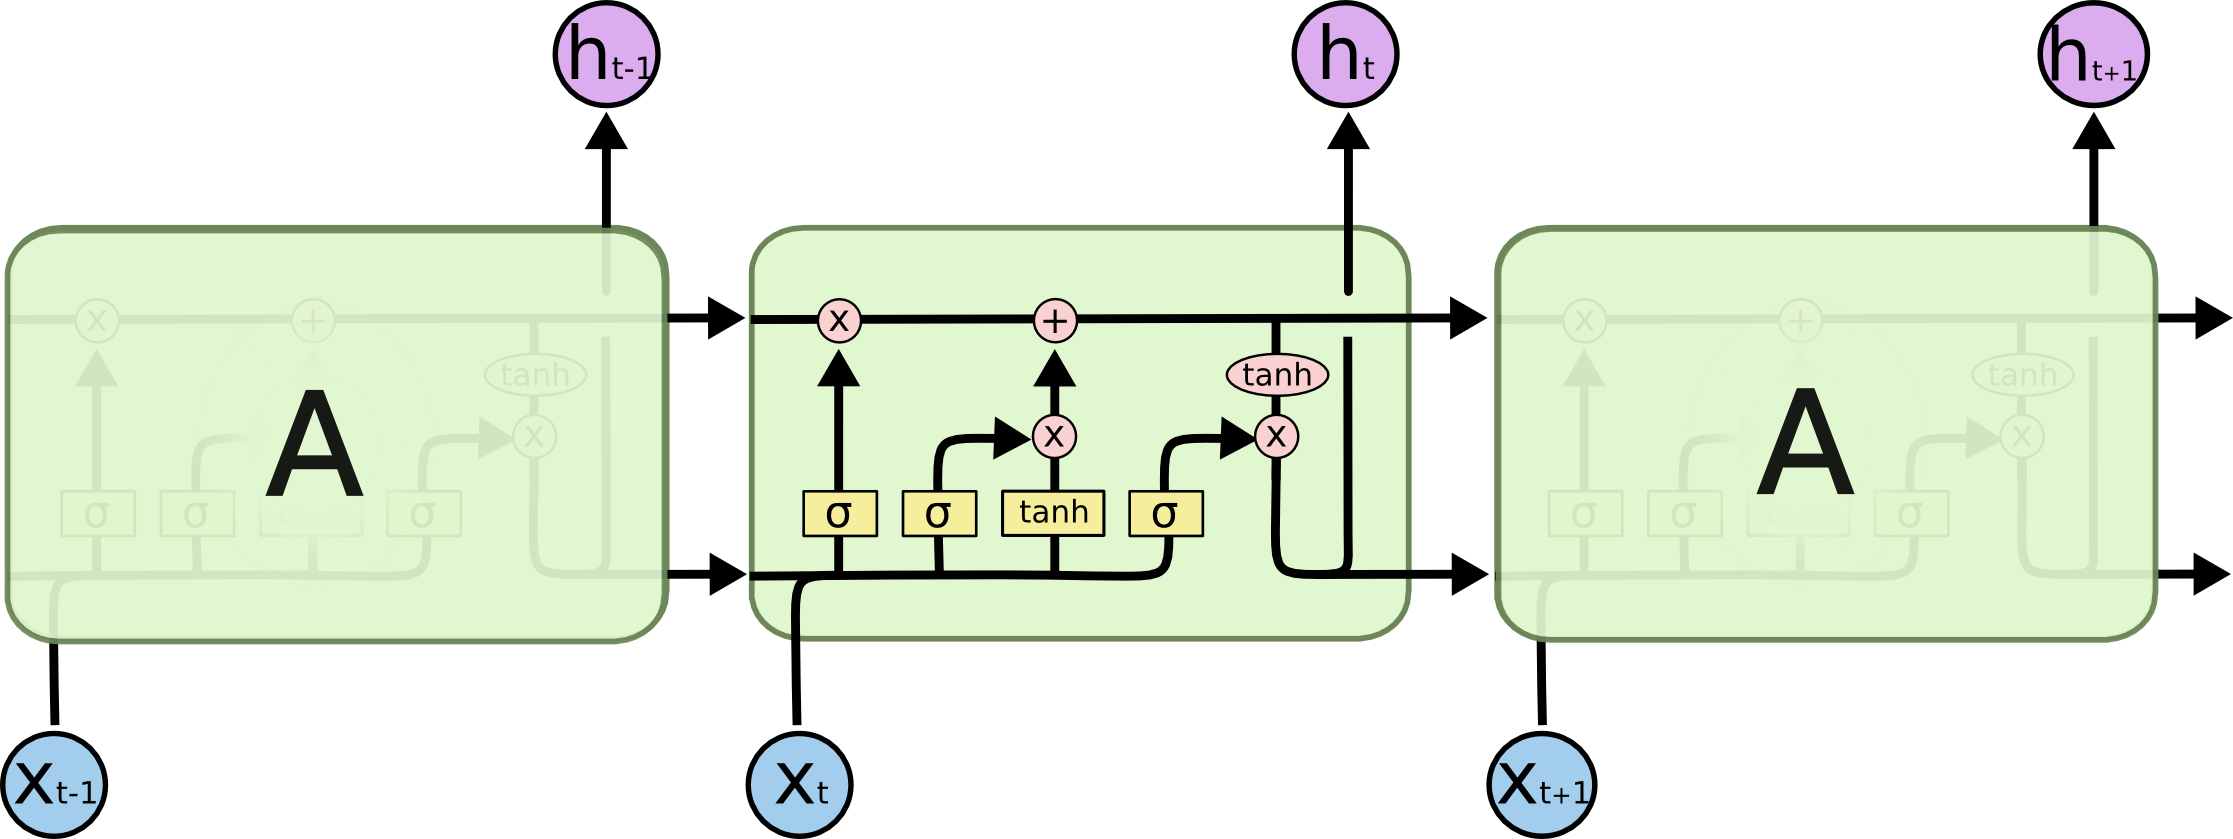
\includegraphics[width=8cm]{bilder/LSTM3-chain}
    \caption{Reihe von LSTM-Zellen mit entsprechenden Gates \citep{lstmexplained}}
\end{figure}

\pagebreak

\section{Transformer}\raggedbottom \label{transformer}
Transformer sind eine spezifische Encoder-Decoder Deep Learning Architektur, die insbesondere im Natural Language Processing eingesetzt wird. 
Basierend auf Attention Layern ermöglichen Transformer die Leistung bei vielen NLP Anwendungen stark zu steigern. 
Ein großer Vorteil von Transformermodellen ist die Parallelisierbarkeit. 
Hierdurch lassen sich extrem große Sprachmodelle, wie zum Beispiel BERT (\textbf{B}idirectional \textbf{E}ncoder \textbf{R}epresentations from \textbf{T}ransformers) oder GPT-2 (\textbf{G}enerative \textbf{P}re-trained \textbf{T}ransformer-2) auf Basis von Transformern trainieren. 
Beide Modelle erzielen in den unterschiedlichsten Benchmarks hervorragende Ergebnisse \citep{DBLP:journals/corr/abs-1810-04805}.

Transformermodelle sind Sequence-To-Sequence Modelle, die aus einem Encoder und einem Decoder bestehen.
Die vortrainierten Sprachmodelle BERT und GPT-2 lassen sich auf spezielle Aufgabenbereiche finetunen.


\subsection{Transformer Encoder / Decoder}
Transformer verwenden eine Encoder - Decoder Struktur. Der Encoder wandelt eine Eingabesequenz $(x_1,\ldots,x_n)$ in eine kontinuierliche Übergangsrepräsentation $z=(z_1, \ldots, z_n)$ um. 
Mit dieser Übergangsrepräsentation $z$ kann anschließlich vom Decoder eine Ausgabesequenz $(y_1, \ldots, y_n)$ generiert werden.
Der Transformer Decoder generiert Textsequenzen autoregressiv und bezieht somit für die Berechnung des nächsten Ausgabetokens die vorherigen Tokens als Eingabe mit ein.


\begin{figure}[h]
    
    \centering
    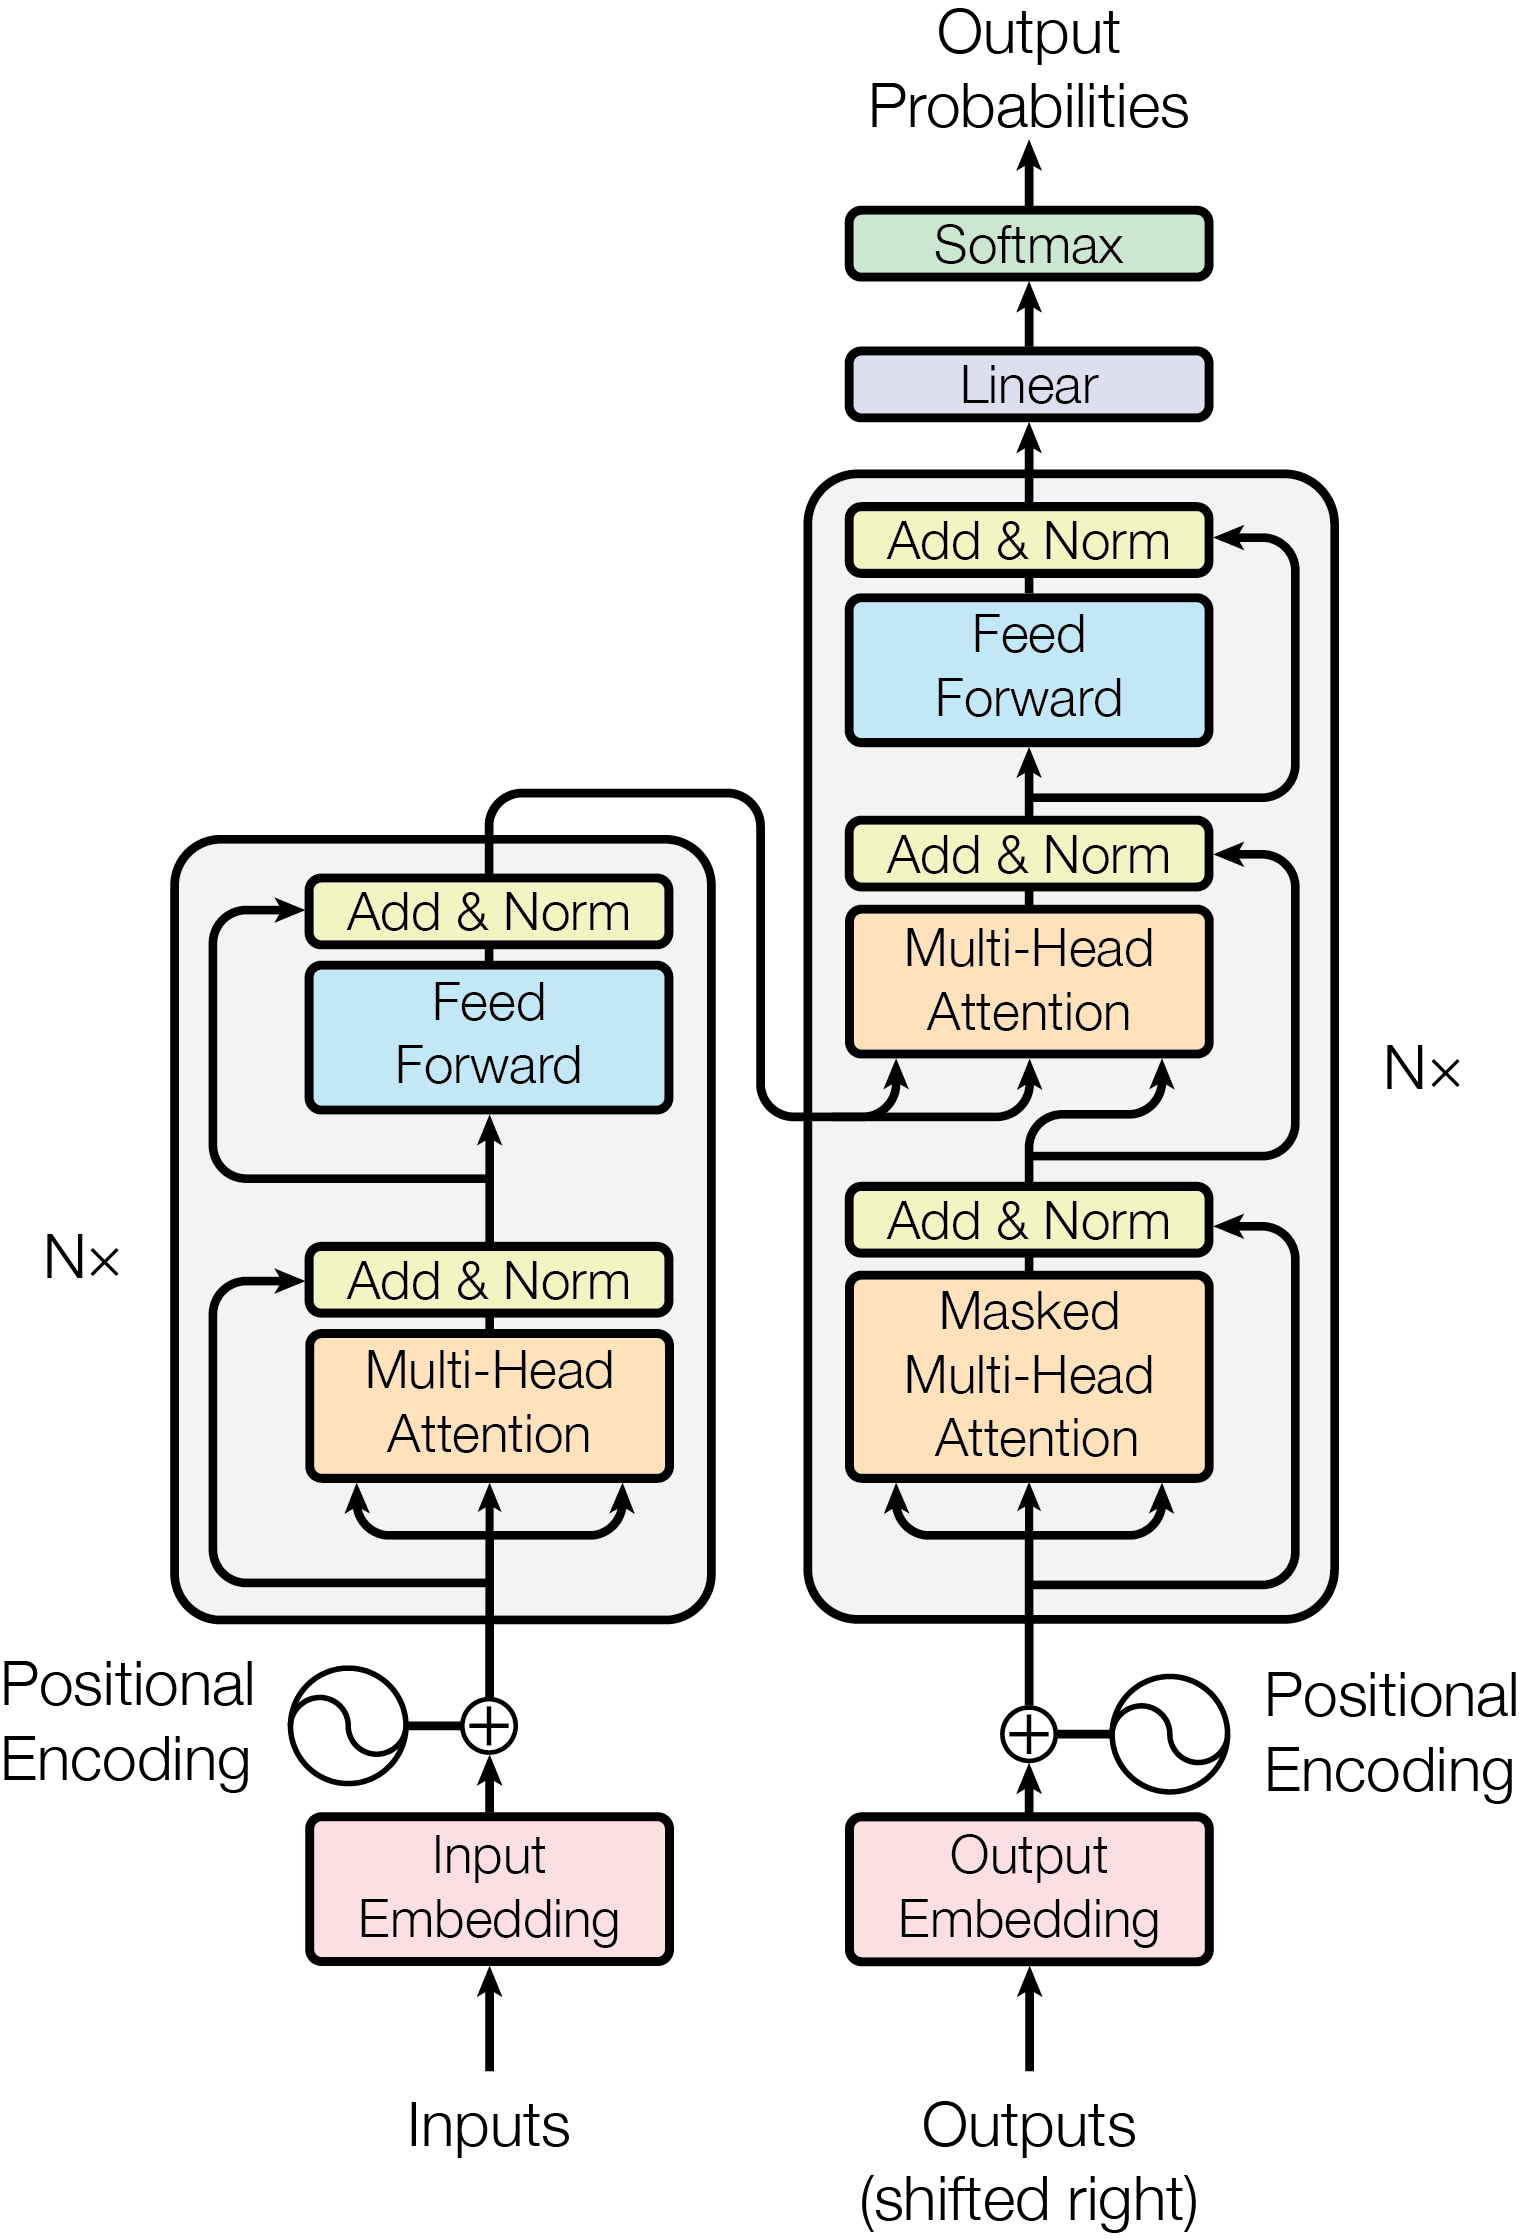
\includegraphics[width=6.3cm]{bilder/Transformer-Encoder-Decoder}
    \caption{Transformer Encoder (links) und Transformer Decoder (rechts) \citep{AttentionIALYN}}
    \label{transformerfig}
\end{figure}

Abbildung \ref{transformerfig} stellt die Architektur und den Datenfluss durch die verschiedenen Layer von Transformer Encodern und Transformer Decodern dar. 
Grundsätzlich bestehen sowohl der Encoder sowie auch der Decoder aus aufeinanderfolgenden Multi-Head Attention-Layern gefolgt von Fully-Connected Feed-Forward-Netzen \citep{AttentionIALYN}.


Die Transformer Encoder Blöcke verwenden Self-Attention-Layer und beziehen damit ihre Eingabe vollständig aus der Ausgabe des vorherigen Layers. 
Die meisten Modelle verwenden mehrere Transformer Encoder Blöcke und Transformer Decoder Blöcke sequentiell hintereinander.

Nach Encodierung der Eingabesequenzen durch den Transformer Encoder wird die Ausgabe in Attention Key- und Value-Vektoren umgewandelt.
Diese Attentionvektoren werden vom Transformer Decoder in den Encoder-Decoder Attention Layern verwendet.
Im Gegensatz zu den Self-Attention-Layern der Encoder verwendet der Decoder hier die Ausgabe des Encoders im Attention-Layer in den Berechnungen mit, um sich auf die korrekten Stellen im Input bei der Generierung der finalen Ausgabesequenz zu fokussieren.


%Stack
%encoder-decoder attention




\subsection{Attention-Layer} %Attnetnion nicht self attention
\label{attention}
Durch die Attention-Layer von Transformermodellen lassen sich relevante Informationen erkennen und das Modell lässt sich auf diese fokussieren. 
Der Attention-Layer innerhalb des Transformers berechnet die Relevanz von Values zu bestimmten Keys und Queries. 

Falls Attention-Layer ihre gesamte Eingabe wie bei Transformer Encodern aus einer Datenquelle beziehen, handelt es sich um Self-Attention-Layer.
Bei Self-Attention-Layern werden die Query- $(Q)$, Key- $(K)$ und Value- $(V)$ Vektoren aus dem Eingabevektor $(X)$ durch Multiplikation mit erlernten Gewichtsmatrizen $(W)$ generiert \citep{AttentionIALYN}. 
\begin{equation}
    Q = X \times W^{Q}, K = X \times W^{K}, V = X \times W^{V}
\end{equation}
Durch ein Dot-Product zwischen Query- und Key-Vektoren der entsprechenden Eingabewörtern mit anschließender Softmax Normalisierung lässt sich ein Score errechnen, der den Fokus im Valuevektor auf das jeweilige Wort gewichtet \citep{AttentionIALYN}.
\begin{equation}
    \label{attentioneq}
    Attention(Q,K,V) = Softmax(\frac{Q\times K^T}{\sqrt{d_k}})\times V
\end{equation}
In Gleichung \ref{attentioneq} werden die Berechnungen an den Matrizen $Q$ für die Queries, $K$ für die Keys und $V$ für die entsprechenden Values durchgeführt. Als Skalierungsfaktor wird $\sqrt{dk}$ , die Dimension der Key Vektoren verwendet, um einen stabilen Gradienten zu erhalten. 

\pagebreak
Attention Funktionen lassen sich parallel ausführen. Diese Eigenschaft nutzen Transformermodelle aus und verwenden Multi-Head Attention Layer, um mehrere Attention Funktionen parallel auszuführen.
Es werden parallel $h$ voneinander unabhängige Attention Layer ausgeführt, die ihre einzelnen Ergebnisse für die Weiterverarbeitung aneinanderfügen und linear in die gewünschte Dimension transformieren. 
\begin{equation}
    \label{multiatteq}
    \begin{split}
    MultiHeadAttention(Q,K,V) &= [head_1, \ldots, head_h] \times W^{O} \\
    \text{mit } head_i &= Attention(QW_i^Q,KW_i^K,VW_i^V)
    \end{split}
\end{equation}
In Gleichung \ref{multiatteq} wird deutlich, dass die unterschiedlichen Attention-Heads voneinander unabhängig sind. Hierdurch können sich die einzelnen Attention-Heads auf unterschiedliche Merkmale in den Daten fokussieren.



    


\subsection{\textbf{B}idirectional \textbf{E}ncoder \textbf{R}epresentations from \textbf{T}ransformers}
BERT (\textbf{B}idirectional \textbf{E}ncoder \textbf{R}epresentations from \textbf{T}ransformers) ist ein von Google \citep{DBLP:journals/corr/abs-1810-04805} entwickeltes Encoder-Sprachmodell, welches sich durch die bidirektionale kontextuelle Einbettung von Worten auszeichnet.
Bei der Veröffentlichung von BERT konnten in vielen NLP Benchmarks Bestleistungen erzielt werden \citep{DBLP:journals/corr/abs-1810-04805}. 

BERT zeichnet sich ebenfalls durch die Möglichkeit des Transfer Learnings aus. Es existieren vortrainierte BERT-Sprachmodelle, die jeweils auf spezifische Aufgaben finegetuned werden können.

Die Modellarchitektur von BERT sind sequentielle Transformerencoderlayer. Das Basis BERT-Modell verwendet 12 Transformerencoderblöcke mit jeweils 12 Multi-Attention-Heads und einer Hidden-Size von 768.
BERT wird mit den beiden Pretrainings Aufgaben Masked Language Modeling und Next Sentence Prediction vortrainiert. Durch den besonderen Trainingsprozess betrachtet BERT Sequenzen von links und rechts gleichzeitig also bidirektional. Einige andere Verfahren betrachten Sequenzen nur einseitig beziehungsweise kombinieren zwei einseitige Betrachtungen wie zum Beispiel ELMO \citep{elmo} und haben demnach keine tiefe bidirektionale Repräsentation der Sequenzen.

Beim Masked Language Modeling werden die bidirektionalen Repräsentationen trainiert, indem zufällig 15\% der Worttokens in einer Sequenz gegen ein \textbf{[MASK]} Token ersetzt werden. Das Trainingsziel ist, die maskierten Tokens korrekt vorherzusagen.
Zum Verständnis der Zusammenhänge zwischen den Sätzen wird beim Next Sentence Prediction Pretrainingsschritt vorhergesagt, ob ein zu 50\% zufällig gewählter Satz B auf Satz A folgt \citep{DBLP:journals/corr/abs-1810-04805}.

\pagebreak
\subsection{\textbf{G}enerative \textbf{P}re-trained \textbf{T}ransformer-2}
GPT-2 (\textbf{G}enerative \textbf{P}re-trained \textbf{T}ransformer-2) ist ein von OpenAI \citep{radford2019language} veröffentlichtes autoregressives Sprachmodell auf Basis von Transformerdecodern.
Autoregressive Sprachmodelle generieren Textsequenzen, indem sie einzeln Tokens generieren und diese an die Eingabesequenz anhängen. Die neue verlängerte Textsequenz wird erneut als Eingabe zur Generierung genutzt.
Als generatives Modell erzielt es hervorragende Ergebnisse beim Generieren von kongruenten Textpassagen.

GPT-2 small besteht aus 12 sequentiellen Transformerdecodern.
Um die autoregressiven Eigenschaften beizubehalten, verwendet GPT-2 Masked Self-Attention Layer. 
Durch die Masked Self-Attention Layer kann das GPT-2 Modell beim Training im Gegensatz zu BERT lediglich die bereits bekannten Tokens betrachten.
%So lassen sich nacheinander jeweils einzelne nachfolgende Tokens zu einer Eingabesequenz generieren. 
%Im nächsten Schritt wird diese Eingabesequenz und das generierte Token als nächste Eingabe verwendet.

Zur Generierung von Textpassagen kann GPT-2 unkontrolliert Samples aus einer leeren Eingabesequenz generieren.
Kontrolliert werden kann die Generierung durch das Festlegen einer spezifischen Starteingabe an die GPT-2 generierte Tokens anfügt.
Weiterhin kann GPT-2 auf einen spezifischen Datensatz finegetuned werden, um so die zu erwartende Ausgabe zu beeinflussen.
Während der Generierung selbst lässt sich die Generierung allerdings nicht kontrollieren.

GPT-2 verwendet zur Tokenisierung das BytePairEncoding Verfahren \citep{bytepairencoding}.
Das Pretraining von GPT-2 wurde auf einem Datensatz mit ca. 8 Millionen Webseiten durchgeführt, mit der Aufgabenstellung jeweils in Texten das nächste Token vorherzusagen.



\pagebreak

\section{Variational Autoencoder}\raggedbottom
\label{vae}
Variational Autoencoder (VAE) \citep{kingma2014autoencoding} gehören zu den probabilistischen generativen Modellarchitekturen. 
Generative Modelle, insbesondere auch Variational Autoencoder, zeigen hervorragende Möglichkeiten auf, hochrealistische Daten wie zum Beispiel Bilder, Texte oder Audios zu generieren.
Generative Modelle versuchen die Merkmale und Verteilung eines Datensatzes zu verstehen und anschließend neuartige Datenbeispiele, die ähnlich zum Trainingsdatensatz sind zu generieren.

Autoencoder sind neuronale Netze, die trainiert werden, um Eingabedaten zu komprimieren und anschließend zu rekonstruieren. 
Sie bestehen aus einem Encoder $\mathbf{E}:\mathbb{R}^n \rightarrow \mathbb{R}^m$ und einem Decoder $\mathbf{D}:\mathbb{R}^m \rightarrow \mathbb{R}^n$, wobei der Encoder versucht, eine komprimierte Darstellung $c \in \mathbb{R}^{m}$ für die Eingabedaten $x \in \mathbb{R}^{n}$ im Latentspace zu finden. Die komprimierte Darstellung im Latentspace wird vom Decoder rekonstruiert mit dem Ziel, eine möglichst identische Rekonstruktion zur Eingabe $x \in \mathbb{R}^{n}$ zu erzeugen.
Um stets eine komprimierte Darstellung im Latentraum zu erhalten und nicht eine Identitätsabbildung für den Encoder und Decoder wird die Dimension der Latentrepräsentation niederiger als die Eingabedimension gewählt, also $m<n$ \citep{introVAE}. 

Da Autoencoder nur einen diskreten Latentraum erzeugen existieren im Latentraum viele leere Stellen, wodurch Interpolation durch den Latentraum zur Rekonstruktion neuer Ausgaben kaum möglich ist.
%Autoencoder erzeugen nur einen diskreten Latentraum, wodurch Interpolation durch den Latentraum zur Rekonstruktion neuer Ausgaben kaum möglich ist, da im Latentraum viele leere Stellen existieren. 
Dies ist darauf zurückzuführen, dass ein Autoencoder auf möglichst geringen Verlust beim Encodieren und Decodieren trainiert wird und somit keinen Wert auf die Organisation des Latentraums legt. 
%Somit führt die fehlende Regularisierung der einzelnen Datenpunkte oft zu Overfitting.

Im Gegensatz zu Autoencodern verwenden Variational Autoencoder einen probabilistischen Ansatz, um Datenpunkte $x_i$ eines Datensatzes $X$, der durch die unbekannte Wahrscheinlichkeitsfunktion $P(\mathbf{X})$ beschrieben wird, im Latentraum $Z$ zu repräsentieren. 
Die Architektur und der probabilistische Ansatz wird in Abbildung \ref{vae_model} dargestellt.
Für den Datensatz $X$ mit Datenpunkten $x_i$ wird angenommen, dass ein generatives Modell mit den Parametern $\theta$ existiert, welches mittels Latentvektor $z_i$ diesen Datenpunkt $x_i$ generieren kann.

\begin{figure}[h]
    \centering
    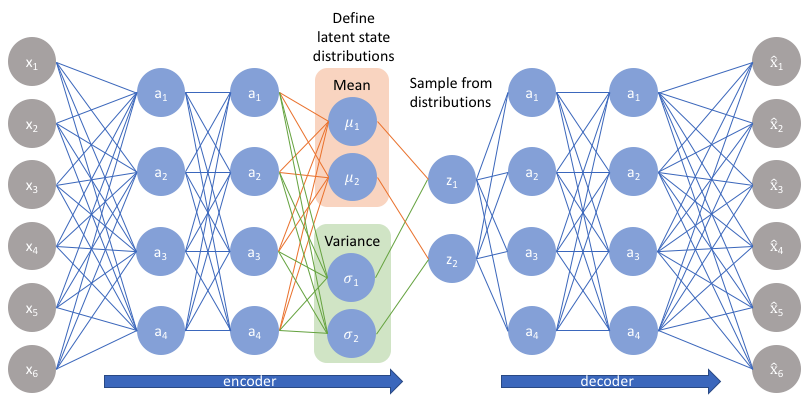
\includegraphics[width=13.2cm]{bilder/vae}
    \caption{Variational Autoencoder Modellarchitektur \citep{jordan_2018}}
    \label{vae_model}
\end{figure}



%only for pagebreak
Dieser generative Teil des Variational Autoencoders ist der Decoder des  Netzes, welcher approximativ versucht, die Daten als Verteilung $p_\theta (\mathbf{x})$ zu modellieren.
\begin{equation}
    \label{px}
p_\theta (\mathbf{x}) = \int_{\mathbf{z}} p_\theta (\mathbf{x\mid z}) p_\theta (\mathbf{z}) dz
\end{equation}
In Gleichung \ref{px} wird für $p_\theta (\mathbf{z})$ die A-priori-Wahrscheinlichkeit angenommen und für $p_\theta (\mathbf{x\mid z})$ die Likelihood. Der Decoder zieht demnach eine Latentvariable $z$ aus der A-priori-Menge $p_\theta (\mathbf{z})$ und berechnet mit der Likelihood $p_\theta (\mathbf{x\mid z})$ Datenpunkte $x$ \citep{vae2}.

%Die inferierten Latentvariablen für die bekannten Datenpunkte $X$ lassen sich über die A-posteriori-Wahrscheinlichkeit $p_\theta (\mathbf{z\mid x})$ aus Gleichung \ref{posteriori} herleiten. 
Die Latentvariablen für die bekannten Datenpunkte $X$ lassen sich über die A-posteriori-Wahrscheinlichkeit $p_\theta (\mathbf{z\mid x})$ aus Gleichung \ref{posteriori} bestimmen. 
\begin{equation}
    \label{posteriori}
    p_\theta (\mathbf{z\mid x}) = \frac{p_\theta (\mathbf{x\mid z}) p_\theta (\mathbf{z})}{p_\theta(\mathbf{x})}
\end{equation}

%Die Berechnung von $p_\theta(x)$ ist meistens nicht möglich. Demnach lässt sich auch $p_\theta (z|x)$ nicht trivial berechnen. 
Der Encoder des Variational Autoencoder approximiert die A-posteriori-Wahrscheinlichkeit durch ein Inferenzmodell $q_\phi (\mathbf{z\mid x})$, da sich $p_\theta (\mathbf{z\mid x})$ nicht trivial berechnen lässt.
Die Parameter $\phi$ des Encoders werden optimiert, um mit $q_\phi (\mathbf{z\mid x}) \approx p_\theta (\mathbf{z\mid x})$ die wahre A-posteriori-Verteilung zu approximieren, indem die Kullback-Leibler-Divigenz zwischen den beiden Wahrscheinlichkeiten minimiert wird, wie in Abschnitt \ref{elbo} beschrieben.



% Der Encoder des Variational Autoencoder encodiert die Eingaben in jeweils eine multivariate Verteilung von der anschließend Latentvektoren $z_i$ gezogen werden. 
% Die Latentvektoren werden anschließend vom Decoder decodiert und der Rekonstruktionsfehler zurückgegeben.
% %Normalerweise werden für die Encodierteverteilung 
% %Normalverteilung Regalusierung erklären https://towardsdatascience.com/understanding-variational-autoencoders-vaes-f70510919f73




% Die Beziehungen zwischen den Eingabedaten $x$ und den Latentvektoren $z$ sind wie folgt definiert, wobei $\phi$ die Parameter des Encoders und $\theta$ die Parameter des Decoders sind:
% \begin{itemize}
% \item Prior $p_\theta (z)$
% \item Likelihood $p_\theta (x|z)$
% \item Posterior $p_\theta (z|x)  \approx q_\phi (z|x)$
% \end{itemize}
% %ANDERS AUFSCHREIBEN

% Da die Posterior Verteilung $p_\theta (z|x)$ nicht bestimmt werden kann, approximieren wir diese mit $q_\phi (z|x)$ unter Verwendung der Variationsinferenzmethode zur Minimierung der Kullback-Leibler-Divergenz, wie in Abschnitt \ref{elbo} beschrieben.

% Um mittels Variational Autoencoder neue Datenobjekte zu samplen wird zunächst mit der Prior-Verteilung $p_\theta (z)$ ein neuer Latentvektor $\hat{z}$ gezogen. Anschließend lässt sich ein neues Datenobjekt $\hat{x}$ mit der Verteilung $p_\theta (x|z=\hat{z})$ generieren.
\subsection{Evidence Lower Bound}
%https://lilianweng.github.io/lil-log/2018/08/12/from-autoencoder-to-beta-vae.html#contractive-autoencoder
%https://openreview.net/forum?id=Sy2fzU9gl
%https://arxiv.org/pdf/1312.6114.pdf
%http://mediatum.ub.tum.de/doc/1547089/1547089.pdf
%https://pub.tik.ee.ethz.ch/students/2018-FS/MA-2018-22.pdf
%https://mediatum.ub.tum.de/doc/1547089/file.pdf
%https://www.jeremyjordan.me/variational-autoencoders/
%https://towardsdatascience.com/understanding-variational-autoencoders-vaes-f70510919f73
%https://arxiv.org/pdf/1906.02691.pdf
%https://arxiv.org/pdf/1903.10145.pdf
%https://ichi.pro/de/generative-modellierung-mit-variational-auto-encoder-vae-277371603749134
%https://xyang35.github.io/2017/04/14/variational-lower-bound/

\label{elbo}
Die Lossfunktion von Variational Autoencodern ist die \textbf{E}vidence \textbf{L}ower \textbf{Bo}und (ELBO).
Bei Variational Autoencodern ist das Optimierungsziel die gleichzeitige Minimierung des Rekonstruktionsfehlers des generativen Modells $\theta$ zwischen Eingabe- und Ausgabedaten sowie die Approximation von $p_\theta (\mathbf{z\mid x})$ mit $q_\phi (\mathbf{z\mid x})$ durch Minimierung der Kullback-Leibler-Divergenz$D_{KL}(q_\phi(\mathbf{z\mid x})\parallel p_\theta(\mathbf{z\mid x}))$.
Für eine beliebige Wahl der Decoder Parameter $\phi$ gilt \citep{introVAE}:
\begin{align}
    log(p_\theta(\mathbf{x})) &= \mathbb{E}_{ q_\phi(\mathbf{z\mid x}) } [log( p_\theta(\mathbf{x}) )] \nonumber \\
    &= \mathbb{E}_{q_\phi( \mathbf{z\mid x} )} \Bigl[ log \Bigl[ \tfrac{ p_\theta(\mathbf{x,z}) }{ p_\theta(\mathbf{z \mid x}) } \Bigr] \Bigr] \nonumber \\
    &= \mathbb{E}_{q_\phi( \mathbf{z\mid x} )} \Bigl[ log \Bigl[ \tfrac{ p_\theta(\mathbf{x,z}) }{ q_\phi( \mathbf{z\mid x} ) } \tfrac{ q_\phi( \mathbf{z\mid x} ) }{ p_\theta(\mathbf{z \mid x}) }\Bigr] \Bigr] \nonumber \\
    &= \underbrace{\mathbb{E}_{q_\phi( \mathbf{z\mid x} )} \Bigl[ log \Bigl[ \tfrac{ p_\theta(\mathbf{x,z}) }{ q_\phi( \mathbf{z\mid x} ) } \Bigr] \Bigr]}_{=\mathcal{L}_{\theta,\phi}(\mathbf{x}) \text{ (ELBO)}} + \underbrace{\mathbb{E}_{q_\phi( \mathbf{z\mid x} )} \Bigl[ log \Bigl[ \tfrac{ q_\phi( \mathbf{z\mid x} ) }{ p_\theta(\mathbf{z \mid x}) }\Bigr] \Bigr]}_{=D_{KL}(q_\phi(\mathbf{z\mid x})\parallel p_\theta(\mathbf{z\mid x}))} \label{elbo4}
\end{align}
In Gleichung \ref{elbo4} ist der erste Term die Evidence Lower Bound und der zweite Teil die Kullback-Leibler Divergenz.
Die Kullback-Leibler Divergenz zwischen $q_\phi(\mathbf{z\mid x})$ und $p_\theta(\mathbf{z\mid x})$ ist nicht negativ und genau null, wenn $q_\phi(\mathbf{z\mid x})$ der wahren A-posteriori-Verteilung entspricht.

\begin{equation}
    \label{dkl}
    D_{KL}(q_\phi(\mathbf{z\mid x})\parallel p_\theta(\mathbf{z\mid x})) \geq 0
\end{equation}

Aus Gleichung \ref{elbo4} wird durch Umformung die Evidence Lower Bound Funktion aufgestellt:
\begin{equation}
    \label{realelbo}
    \mathcal{L}_{\theta,\phi}(\mathbf{x}) = log(p_\theta(\mathbf{x})) - D_{KL}(q_\phi(\mathbf{z\mid x})\parallel p_\theta(\mathbf{z\mid x})) \leq log(p_\theta(\mathbf{x})) 
\end{equation}
Da die Kullback-Leibler Divergenz in Gleichung \ref{dkl} keine negativen Werte annimmt ist die Evidence Lower Bound eine untere Schranke der Log-Likelihood der Datenmenge.
Bei Maximierung der Evidence Lower Bound Funktion in Gleichung \ref{realelbo} wird die Evidenz $log(p_\theta(\mathbf{x}))$ maximiert, wodurch das generative Modell verbessert wird. Ebenfalls wird die Kullback-Leibler Divergenz minimiert, wodurch der Encoder die A-posteriori-Verteilung besser approximieren kann.

Somit wird als Lossfunktion $\mathbf{L}_{\theta,\phi}$ die negative Evidence Lower Bound Funktion gewählt, die es zu minimieren gilt:
\begin{align}
    \mathbf{L}_{\theta,\phi} &= -\mathcal{L}_{\theta,\phi}(\mathbf{x}) = -log(p_\theta(\mathbf{x})) + D_{KL}(q_\phi(\mathbf{z\mid x})\parallel p_\theta(\mathbf{z\mid x}))  \\
    \hat{\theta},\hat{\phi} &= \underset{\theta, \phi}{\arg\min \ } \mathbf{L}_{\theta,\phi}
\end{align}
Diese Lossfunktion erlaubt das simultane Optimieren der beiden Parameter $\theta$ und $\phi$.


% \begin{align*}
%     \small
%     D_{KL}(q_\phi(\mathbf{z\mid x})\parallel p_\theta(\mathbf{z\mid x})) &= \int q_\phi(\mathbf{z\mid x}) \log \frac{q_\phi(\mathbf{z\mid x})}{p_\theta(\mathbf{z\mid x})} \, d\mathbf{z}\\
%     &= \int q_\phi(\mathbf{z\mid x}) \log \frac{q_\phi(\mathbf{z\mid x})p_\theta(\mathbf{x})}{p_\theta(\mathbf{z,x})} \,d\mathbf{z}\\
%     &= \int q_\phi(\mathbf{z\mid x}) \left( \log (p_\theta(\mathbf{x})) + \log \frac{q_\phi(\mathbf{z\mid x})}{p_\theta(\mathbf{z,x})}\right) d\mathbf{z}\\
%     &= \log (p_\theta(\mathbf{x})) + \int q_\phi(\mathbf{z\mid x}) \log \frac{q_\phi(\mathbf{z\mid x})}{p_\theta(\mathbf{z,x})} \,d\mathbf{z}\\
%     &= \log (p_\theta(\mathbf{x})) + \int q_\phi(\mathbf{z\mid x}) \log \frac{q_\phi(\mathbf{z\mid x})}{p_\theta(\mathbf{x\mid z})p_\theta(\mathbf{z})} \,d\mathbf{z}\\
%     &= \log (p_\theta(\mathbf{x})) + E_{\mathbf{z} \sim q_\phi(\mathbf{z\mid x})}(\log \frac{q_\phi(\mathbf{z\mid x})}{p_\theta(\mathbf{z})} - \log(p_\theta(\mathbf{x\mid z})))\\
%     &= \log (p_\theta(\mathbf{x})) + D_{KL}(q_\phi(\mathbf{z\mid x}) \parallel p_\theta(\mathbf{z})) - E_{\mathbf{z} \sim q_\phi(\mathbf{z\mid x})}(\log(p_\theta(\mathbf{x\mid z})))
% \end{align*}
% der \textbf{E}vidence \textbf{L}ower \textbf{B}ound (ELBO).


% ÜBERARBEITEN
\subsubsection{Reparametisierung} %kingma welling
Zum Training des Variational Autoencoder wird mittels Backpropagation der Fehler des Netzwerkes propagiert. Da das Samplen von $z \sim q_\phi(\mathbf{z\mid x})$ nicht deterministisch ist, kann hier keine Backpropagation durchgeführt werden.
Um dennoch Backpropagation verwenden zu können, wird mittels Reparametisierung $z$ durch eine deterministische Funktion $z=f_\phi(x,\epsilon)$ dargestellt mit $\epsilon$ als externe unabhängige Hilfsvariable \citep{kingma2014autoencoding,jordan_2018}. 
Bei einer multivariaten Gaussverteilung für $q_\phi (\mathbf{z\mid x})$ wäre die Reparametisierung wie folgt, wobei $\times$ die elementweise Multiplikation denotiert:
\begin{align}
    \mathbf{z} \sim q_\phi(\mathbf{z\mid x}) = \mathcal{N}(\mathbf{z;\mu,\sigma \mathcal{I}}) \nonumber \\
    \mathbf{z} = \mu + \sigma \times \mathbf{\epsilon} \text{ , mit } \mathbf{\epsilon} \sim \mathcal{N}(0,\mathcal{I}) 
\end{align}

\subsection{Cyclical Annealing Schedule}
\label{cyc_anneal}
Trainieren von Variational Autoencodern als Sprachmodell im Bereich des Natural Language Processing ist aufgrund des KL-Vanishing Problems besonders schwierig.
VAE Sprachmodelle sollen bei der Textgeneration den lokalen Kontext, allerdings auch globale Eigenschaften wie zum Beispiel Thema, Sprachstil oder Stimmung beachten. 
Trotzdem werden von VAE Modellen bei der Generierung oft die globalen Eigenschaften vernachlässigt \citep{cyc_anneal}. 
Dieses Problem ist als KL-Vanishing bekannt, da die KL-Regularisierung des Loss-Terms beim Trainieren von autoregressiven Decodern innerhalb von VAE Sprachmodellen sehr klein wird.
Somit sind die erlernten Features nahezu identisch zu der vorher angenommenen Normalverteilung und der Decoder nutzt keine Latentfeatures bei der Generierung. %https://www.microsoft.com/en-us/research/blog/less-pain-more-gain-a-simple-method-for-vae-training-with-less-of-that-kl-vanishing-agony/ nochmal checken

Abhilfe schafft die Verwendung eines $\beta$-Variational Autoencoder \citep{cyc_anneal} mit zyklischem Erhöhen des $\beta$ Wertes.
$\beta$-Variational Autoencoder sind Variational Autoencoder, die mit einen Lagrangemultiplikator $\beta$ die KL-Divergenz der Loss-Funktion gewichten, um besser separierte Latentfaktoren zu finden.
\begin{equation}
    \mathbf{L}_{\beta} (\beta,\theta,\phi)= -\mathbb{E}_{z\sim q_\phi(\mathbf{z\mid x})}[log p_\theta (\mathbf{x\mid z})]- \beta D_{KL}(q_\phi(\mathbf{z\mid x}) \parallel p_\theta(\mathbf{z})) 
\end{equation}
Falls $\beta = 0$ ist wird das Modell wie ein normaler Autoencoder trainiert, bei $\beta = 1$ wie ein normaler Varitional Autoencoder.

Beim zyklischen Erhöhen wird der $\beta$-Wert des VAE während des Trainings monoton von $\beta=0$ auf zum Ende des Trainings $\beta=1$ in kleinen Abständen erhöht.
So kann beim Training des VAE bei $\beta<1$ zunächst der Fokus darauf gelegt werden, mehr Information für die Rekonstruktion zu erlernen. 
Abschließend enthalten bei $\beta=1$ die vorher trainierten $z$ Vektoren bereits mehr Informationen, die zu einer besseren Anpassung als eine zufällige Initialisierung führen.


\subsection{Optimus}
Optimus (\textbf{O}rganizing \textbf{S}entences via \textbf{P}re-trained \textbf{M}odeling of a \textbf{L}atent \textbf{S}pace) \citep{DBLP:journals/corr/abs-2004-04092} ist ein großes vortrainiertes Deep Latent Variable Modell für natürliche Sprache.
Die Modelarchitektur von Optimus ist ein Variational Autoencoder, der als Encoder BERT und als Decoder GPT-2 verwendet wie in Abbildung \ref{optimus_scheme_fig} zu erkennen ist. 
Verwendet wird jeweils das vortrainierte BERT Base Modell $\phi_{BERT}$ und das vortrainierte GPT-2 Base Modell $\theta_{GPT-2}$ beide mit 12 Layern, 12 Attention Heads und einer Hiddensize von 768. 
\begin{figure}[h]
    \centering
    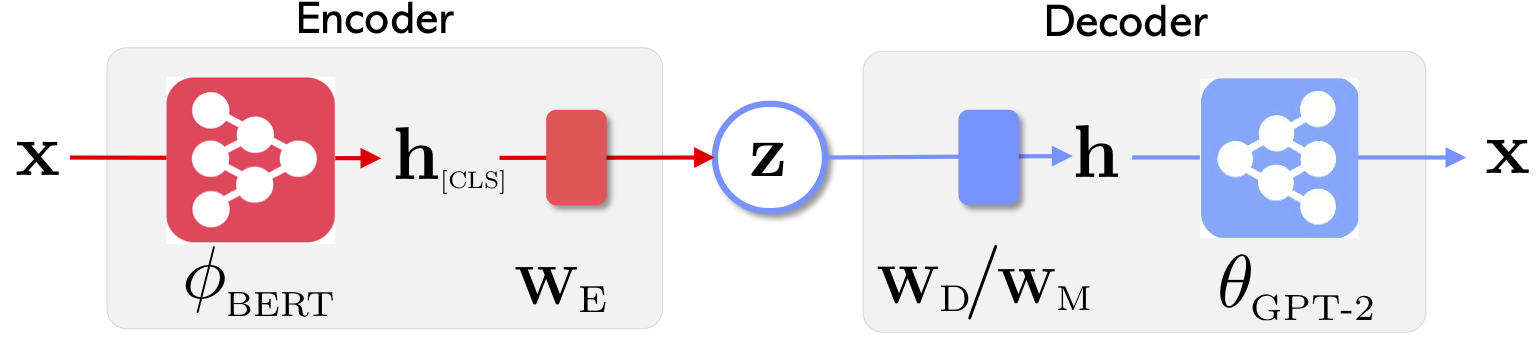
\includegraphics[width=\textwidth]{bilder/optimus_scheme}
    \caption{VAE Modellarchitektur von Optimus mit BERT als Encoder und GPT-2 als Decoder \citep{DBLP:journals/corr/abs-2004-04092}}
    \label{optimus_scheme_fig}
\end{figure}
Trainiert wird Optimus mit dem Ziel, Sätze in einem universellen Latentspace zu organisieren und somit übergreifende semantische Muster für die einzelnen Sätze zu finden.
Somit kann durch gezieltes Verändern des Latentvektors $z$ kontrolliert Text generiert werden. %ÜBERARBEITEN

BERT und GPT-2 über eine VAE Architektur miteinander zu verbinden hat die Herausforderung, die unterschiedlichen Tokenisierungsschemen der einzelnen Modelle zu verwenden und den Latentvektor bei der Textgeneration von GPT-2 zu injizieren. 
Die Eingabetokens von BERT verwenden das WordPiece Embeddings Verfahren \citep{wordpiece} mit einer Vokabulargröße von 28.996 Tokens. 
Die Ausgabe erfolgt über die Byte Pair Encoding Tokenisierung \citep{bytepairencoding} von GPT-2 mit einer Vokabulargröße von 50.260 Tokens. 
Innerhalb des Netzwerkes wird im Latentvektor ein Token durch eine Einbettung $h_{Emb}$, die das Token, die Position und das Segment Embedding wiedergibt, repräsentiert.
Um beim Training den Loss der Rekonstruktionsaufgabe zu berechnen, werden die Sätze mit beiden Tokenisierungen tokenisiert.


Als Latentvektor $z \in \mathbb{R}^P$ wird die gepoolte Ausgabe des letzten Hiddenlayers $h_{[CLS]} \in \mathbb{R}^H$ von BERT mit einer Gewichtsmatrix multipliziert $W_{E} \in \mathbb{R}^{P\times H}$ gewählt. Somit kann ein Latentvektor wie folgt bestimmt werden $z = W_{E}h_{[CLS]}$.

\begin{figure}[h]
    \centering
    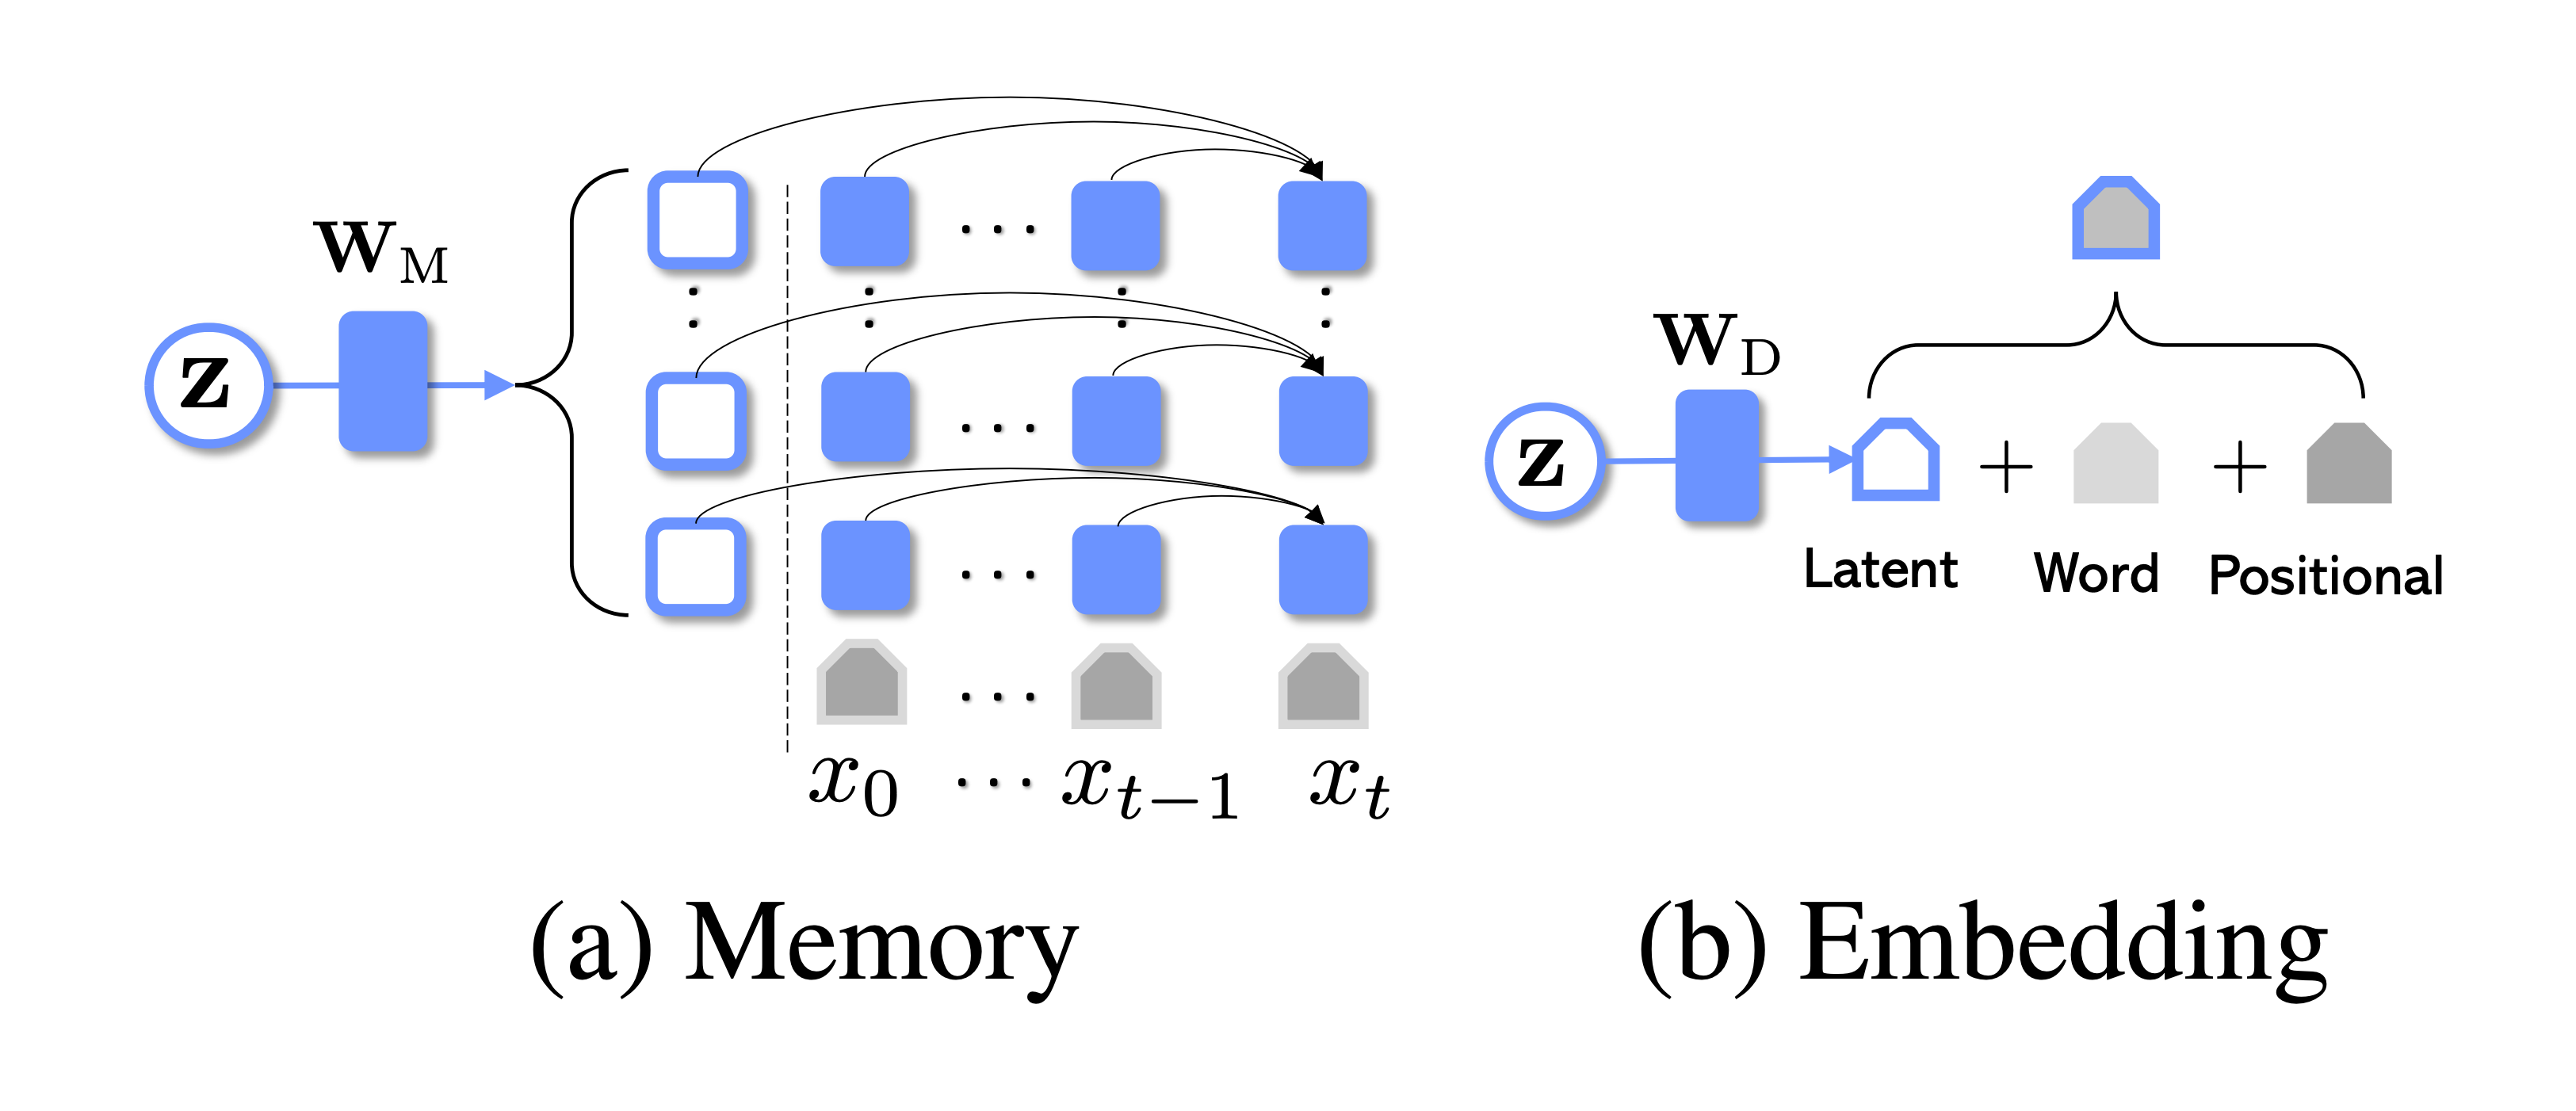
\includegraphics[width=11cm]{bilder/latent_optimus}
    \caption{Methoden, um den Latentvektor in GPT-2 zu injizieren \citep{DBLP:journals/corr/abs-2004-04092}}
    \label{latent_optimus}
\end{figure}

Um mit GPT-2 kontrolliert unter Verwendung des Latentvektors Text zu generieren, kann der Latentvektor entweder als Memoryvektor in die Past-Gewichtsmatrix injeziert oder auf die vorherigen Embeddings addiert werden \citep{DBLP:journals/corr/abs-2004-04092}.

Beim Embedding wird $z$ direkt auf den Embedding Layer addiert. Somit ergibt sich der neue Embedding Layer durch $h_{Emb}^{'} = h_{Emb} + W_D z$ mit der Gewichtsmatrix $W_D \in \mathbb{R}^{H \times P}$.
Der Decoder kann hier die zusätzlichen Informationen des Embeddings im Input und Output Layer verwenden.

Bei der Injezierung von $z$ als Memoryvektor $h_{Mem} \in \mathbb{R}^{L\times H}$ wird der Latentvektor in den Past-Key-Vektor von GPT-2 injeziert. 
Der Past-Key-Vektor beschleunigt normalerweise den Decodiervorgang von GPT-2, da bei einem Decodierungsdurchlauf zu den vorherigen Tokens bereits berechnete Key- und Valuevektoren der Attentionlayern gespeichert und wiederverwendet werden.
Diese Key-, Valuevektoren des Attentionlayers werden durch $h_{Mem} = W_M z$ mit $W_M \in \mathbb{R}^{LH \times P}$ ersetzt. GPT-2 kann so beim Decodieren auf den injezierten Latentvektor bei jeder Attentionberechnung zugreifen.

Die Parameter ${\phi_{BERT}, \theta_{GPT-2}, W_E,W_M,W_D}$ des VAEs werden mittels Cyclical Annealing Schedule \citep{cyc_anneal} trainiert, um das KL Vanishing Problem beim Trainieren eines VAEs zu verhindern.
Die $\beta$ Variable, die wie in Abschnitt \ref{cyc_anneal} dargestellt den KL-Regularisierungs Anteil steuert, wird für einen Trainingsdurchlauf für die erste halbe Menge der Trainingsdaten auf $\beta = 0$ gesetzt. Somit wird zu Beginn lediglich ein Autoencoder trainiert. 
Anschließend wird $\beta$ für das nächste Viertel der Trainingsmenge schrittweise von 0 auf 1 erhöht und für das letzte Viertel der Trainingsmenge auf 1 belassen, um das VAE Modell zu trainieren.

Insgesamt zeigt Optimus gute Ergebnisse in den Bereichen des Language Modeling, der kontrollierten Text Generation und des Language Understanding.


%%%%PAST KEY VEKTOR MATRIX == Vergangenheitsmatrix

\pagebreak
\subsection{\textsc{BiMeanVAE}}
\textsc{BiMeanVAE} ist ein von \citep{coop} vorgestelltes Modell, bestehend aus einem bidirektionalem LSTM Encoder und einem LSTM Decoder. 
Die Hiddensize der einzelnen LSTMs beträgt 512. Nach dem BiLSTM Encoder wird ein Mean Pooling Layer verwendet, um einen Latentvektor $z$ zu erhalten.
\textsc{BiMeanVAE} verwendet die Standard Variational Autoencoder Ziele, das Minimieren des Rekonstruktionsfehlers mit KL-Regularisierung.
Die verwendete Prior Verteilung $p_\theta(z)$ ist die Gausssche Normalverteilung $\mathcal{N}(0,\mathcal{I})$. 
Beim Training wird ebenfalls das in Abschnitt \ref{cyc_anneal} beschriebene Cyclical Annealing Verfahren verwendet, um graduell vom Autoencoder zum Variational Autoencoder Trainingsziel überzuleiten.


\subsection{Latent Space Operationen}
VAEs erlernen bidirektionale Abbildungen zwischen dem Datenraum und ihrem Latentspace. 
Im Latentspace werden Eingabesequenzen von Optimus und \textsc{BiMeanVAE} jeweils durch einen Latentvektor dargestellt.
Die zur Generation verwendeten Latentvektoren können durch arithmetische Operationen verändert werden, wodurch sich die gesampelte Ausgabe des VAEs gezielt verändern und steuern lässt.

Durch die KL-Regularisierung beim Training von VAEs entsteht ein kontinuierlicher Latentspace, wodurch semantisch ähnliche Inhalte im Latentspace nah beieinander organisiert werden.
Somit kann zwischen mehreren Datenobjekten im Latentspace interpoliert werden.

Insbesondere für das kontrollierte Generieren von Bewertungen sind diese Latent Space Operationen, die VAEs ermöglichen, elementar.
So kann zum Beispiel zwischen mehreren Bewertungen interpoliert werden, um eine durchschnittliche Meinung zu generieren.

Sei zum Beispiel $\mathcal{Z}$ die Menge der encodierten Bewertungen zu einer Produktgruppe, so lässt sich aus einer Untergruppe der Vektoren $\mathcal{Z}^{'} \subseteq \mathcal{Z}$ durch Kombinieren eine gute Durchschnittsrepräsentation im Latentvektorraum finden.
Das genaue Vorgehen zum Finden einer solchen Untergruppe wird in Abschnitt \ref{coop_chap} beschrieben
\pagebreak

\section{Datensätze}\raggedbottom
\label{dataset}
%Datensätze mit Gruppentheorie erklären
Zum Training und zur Evaluation von neuronalen Netzen sind große Datensätze erforderlich. 
Zur Lösung der Aufgabenstellung, Durchschnittsrezensionen aus Textbewertungen zu erzeugen, werden Datensätze mit mehreren Bewertungen und Zusammenfassungen zu einem Produkt benötigt.

Es bietet sich an, Bewertungen von großen Webportalen wie Amazon oder Yelp zu verwenden. 
Diese Portale haben zu den unterschiedlichsten Produkten und Dienstleistungen zahlreiche Bewertungen.

Es existieren bereits bestehende Amazon und Yelp Datensätze mit menschlich erstellten Gold-Standard Zusammenfassungen \citep{copycat}. 
Die Variational Autoencoder Modelle lassen sich somit mit den Review Daten mit dem Trainingsziel der Rekonstruktion trainieren, um einen aussagekräftigen Latentraum mit Bewertungen und deren spezifischen Eigenschaften zu erlernen.
Anschließend können die trainierten Modelle auf den respektiven Testdatensätzen evaluiert werden, da jeweils Gold-Standard Zusamenfassungen vorliegen, mit denen sich mittels in Abschnitt \ref{evalmetric} erklärten Metriken die generierten Rezensionen bewerten lassen.

Der Umfang der zum Training und Testen verwendeten Datensätze ist in Tabelle \ref{dataset_table} angegeben.

\begin{table}[!h]
    \centering
    \begin{tabular}{@{}lccc|ccc@{}}
        \toprule
                              &            & \textbf{Amazon} &      &           & \textbf{Yelp} &      \\
                              & Train      & Dev             & Test & Train     & Dev           & Test \\ \midrule
    \# Produkte / Dienstleister & 244.652    &   28            &  32  & 75.988    &  100          &  100    \\
    \# Rezensionen            & 13.053.202 &    224          &   256& 4.658.968 &  800          &  800 \\ \bottomrule
    \end{tabular}
    \caption{Enthaltene Rezensionen der einzelnen Datensätze \citep{coop}}
    \label{dataset_table}
    \end{table}

\subsection{Amazon Datensatz}
Der Amazon Review Datensatz \citep{brazinskas2020-unsupervised} umfasst zahlreiche Rezensionen zu den unterschiedlichsten Produkten, die auf dem Amazon Marktplatz gelistet sind.
Die Rezensionen wurden von Amazon Nutzern erstellt und geben eine unabhängige Meinung über das erworbene Produkt wieder.
Bei Betrachtung der einzelnen Bewertungen fällt auf, dass die meisten Bewertungen von Produkten eher objektiv formuliert sind. 
Die Bewertungen gehen oft auf unterschiedliche Aspekte der Produkte ein und erläutern positive sowie negative Erfahrungen, die auf einzelne Produkteigenschaften zurückzuführen sind.



Die für das Training relevanten Bewertungen wurden aus den Kategorien Kleidung, Schuhe, Schmuck, Elektronikartikeln, Gesundheit- und Pflegeprodukte, Einrichtung und Küchenartikeln gewählt.
Gefiltert wurden die Bewertungen indem Produkte mit einer maximalen Länge von 128 Tokens gewählt wurden und nur Produkte mit über 10 existierenden Bewertungen ausgewählt wurden. 
Die entsprechenden Bewertungen sind bereits in Trainings- und Validierungsdaten gesplittet.

%layout pagebreak
Die Validierungsdaten des Amazon Datensatz sind manuell erstellte Zusammenfassungen, die für den Dev / Test Split im Verhältnis von 28 / 32 vorliegen.
Für jedes Produkt der Validierungsdaten existieren jeweils drei manuell erstellte Referenzzusammenfassungen.
Somit ergibt sich insgesamt ein Trainingsdatensatz mit 244.652 Produkten und den zugehörigen 13.053.202 Bewertungen.
Abbildung \ref{amz_review_example} zeigt exemplarisch eine Rezension zu einem Produkt des Amazon Datensatzes.

\setlength{\fboxsep}{1em}

\begin{figure}[!h]
    \centering
    \scriptsize
    \framebox{

        \parbox{\columnwidth-4\fboxsep}{\textbf{Produkt:} NuGo Protein Bar, Vanilla Yogurt \\ \\ \textbf{Review:} Apart from the obvious nutritional value, the taste was surprisingly better than I anticipated. Normally, if I find soy-based nutritional bars tend to have a chalky or tree-bark-like texture and taste. I dare say, the texture reminds me of a healthy-not-too-sweet 'Rice Krispy Treat'.}

    }
    \caption{Beispiel Bewertung zu einem Produkt des Amazon Datensatzes}
    \label{amz_review_example}
\end{figure}
% Der Datensatz enthält somit diverse Produkte, bei denen jeweils unterschiedliche Eigenschaften wichtig sind.

% Der Amazon Datensatz wurde gefiltert und es wurden nur Produkte mit mindestens 10 Bewertungen, die eine Länge zwischen 20 und 70 Wörter haben, ausgewählt.
% Des Weiteren enthält der Amazon Datensatz manuell erstellte Zusammenfassungen, die für den Dev / Test Split im Verhältnis von 28 / 32 vorliegen.
% Die meisten Bewertungen im Amazon Datensatz sind eher objektiv formuliert und beziehen sich auf die einzelnen Produktspezifischen Eigenschaften.


% Der Amazon Review Datensatz \citep{brazinskas2020-unsupervised} umfasst 4.807.338 Bewertungen zu 192.742 Produkten. 
% Die Bewertungen wurden aus den Kategorien Kleidung, Schuhe, Schmuck, Elektronikartikel, Gesundheit- und Pflegeprodukte, Einrichtung und Küchenartikeln gewählt.
% Gefiltert wurden die Bewertungen indem eine maximale Länge von 150 Tokens gewählt wurde und nur Produkte mit über 50 existierenden Bewertungen ausgewählt wurden. 
% Die entsprechenden Bewertungen sind bereits in Trainings- und Validierungsdaten gesplittet.
% Der Datensatz enthält somit diverse Produkte, bei denen jeweils unterschiedliche Eigenschaften wichtig sind.

% Der Amazon Datensatz wurde gefiltert und es wurden nur Produkte mit mindestens 10 Bewertungen, die eine Länge zwischen 20 und 70 Wörter haben, ausgewählt.
% Des Weiteren enthält der Amazon Datensatz manuell erstellte Zusammenfassungen, die für den Dev / Test Split im Verhältnis von 28 / 32 vorliegen.
% Die meisten Bewertungen im Amazon Datensatz sind eher objektiv formuliert und beziehen sich auf die einzelnen Produktspezifischen Eigenschaften.

\subsection{Yelp Datensatz}
Der Yelp Review Datensatz \citep{meansum} enthält Rezensionen zu unterschiedlichen Gastronomiebetrieben und Unternehmen der Bewertungsplattform Yelp. 
Die von den Yelpnutzern erstellten Bewertungen unterscheiden sich von den Amazon Bewertungen durch mehr Subjektivität in den Bewertungen.
Die Bewertungen enthalten wesentlich mehr persönliche Details und Erfahrungen der Nutzer.
Das Variational Autoencoder Modell hat hier die Aufgabe, wichtige Informationen zu extrahieren und unwichtiges Rauschen in den Daten herauszufiltern, um eine gute Durchschnittsrepräsentation zu bestimmen.
Insbesondere in den Yelp Reviews befinden sich teilweise unnötige Zusatzinformationen, die nicht zur Bewertung der Dienstleistung an sich beitragen, wie zum Beispiel das Erwähnen von privat ausgetragenen Geburtstagsfeiern. 



Der Yelp Review Datensatz wurde ebenfalls nach einer maximalen Länge von 128 Tokens mit mindestens 10 existierenden Bewertungen je Unternehmen gefiltert und besteht somit aus 4.658.968 Bewertungen zu 75.988 Unternehmen, die bereits in Trainings- und Validierungsdaten gesplittet sind. 
Zusätzlich enthält der Datensatz 200 menschlich durch Amazon Mechanical Turk (AMT) Arbeiter erstellte Zusammenfassungen, die zu einem Dev / Test Verhältnis von 100 / 100 gesplittet werden. 
Bei dem Yelp Datensatz liegt für jede der 200 Dienstleistungen der Validierungsdaten lediglich eine Referenzzusammenfassung vor.
Abbildung \ref{yelp_review_example} zeigt beispielhaft eine Bewertung zu einer Konditorei des Yelp Datensatzes.

\begin{figure}[!h]
    \centering
    \scriptsize
    \framebox{

        \parbox{\columnwidth-4\fboxsep}{\textbf{Dienstleister Id:} 87YsVbCN\_kfzheY79Fzjkg \\ \\ \textbf{Review:} Great experience! Went cake tasting for our wedding and Jessica was a huge help!! She brought out the tastings for us after giving us time to look through their amazing book. She explained every cake and filling and had great recommendations for mixing the fillings. The champagne cake with cream cheese filling was amazing!! Chose our cake and design within an hour. Great service and knowledge. Thank you Jessica!}

    }
    \caption{Beispiel Bewertung zu einer Konditorei des Yelp Datensatzes}
    \label{yelp_review_example}
\end{figure}
\pagebreak

\section{Multi-Document Summarization}
In den letzten Jahren erzielten unterschiedliche Verfahren große Fortschritte beim automatisierten Zusammenfassen von mehreren Dokumenten zu einem repräsentativen Dokument.
Im Gegensatz zum normalen Zusammenfassen von einzelnen Dokumenten enthalten beim Multi-Document Zusammenfassen mehrere Dokumente über ein Thema viele redundante Informationen, die so gefiltert werden müssen, dass redundante Informationen nur einmal im Ausgabedokument dargestellt werden.
Ebenfalls ist das Verarbeiten von widersprüchlichen Informationen eine große Herausforderung bei der Zusammenfassung von mehreren Dokumenten.
Das Ziel von Multi-Document Summarization ist das zusammengefasste Repräsentieren der wichtigen Aspekte aller Dokumente in einem einzelnen Dokument, um einen guten allgemeinen Überblick zu schaffen.

Im weiteren Verlauf werden Multi-Document Summarization Systeme zur Zusammenfassung von Bewertungen verwendet.
Sei $R= \{x_i \}$ ein Datensatz von Bewertungen mit einzelnen Bewertungen $x=(x_1,...,x_{\| x \|})$, die aus einer Sequenz aus Wörtern bestehen.
Ziel ist es für ein gegebenes Produkt $p$ und die entsprechenden Bewertungen $R_p \subseteq R$ eine Zusammenfassung $s_p$ zu generieren, die alle relevanten Informationen faktisch korrekt representiert.


Insbesondere im Bereich der Multi-Review Summarization existieren viele unterschiedliche Ansätze.
Zum einen existieren extraktive Ansätze, wie zum Beispiel LexRank \citep{lexrank}, ein unüberwachter Algorithmus, der repräsentative Sätze für eine Bewertung basierend auf ihrer Zentralität in einem TF-IDF gewichteten Graphen selektiert.
Zum anderen existieren abstraktive Ansätze wie zum Beispiel MeanSum \citep{meansum}, CopyCat \citep{copycat} oder COOP \citep{coop}, die generative Ansätze verwenden, um neuartige Sätze in den Bewertungen zu erzeugen.

Die abstraktiven Modelle basieren auf Autoencoder Architekturen. Es wird ein Encoder $E_\phi : X \rightarrow Z$ verwendet, um Textrepräsentationen in einen Latentvektor im Latentraum $Z$ umzuwandeln.
Aus den Latentvektoren $z$ kann anschließend unter Verwendung von einem Decoder $D_\theta : Z \rightarrow \hat{X}$ eine Textrepräsentation generiert werden.


MeanSum ist ein Autoencoder Modell \citep{meansum} mit LSTM Encoder und Decoder und errechnet zur Zusammenfassung von Bewertungen den Durchschnitt von den einzelnen Latentvektoren der Bewertungen $z_p = \bar{z} \text{, mit } z=\{z_{p_1},z_{p_2},...z_{p_k}\}$.
Von diesem Durchschnittslatentvektor $z_p$ wird anschließend eine Bewertung generiert. 


CopyCat basiert auf einem Variational Autoencoder Modell \citep{copycat}, welches GRU Encoder und Decoder verwendet. 
Für jede Gruppe von Bewertungen berechnet CopyCat einen Latentvektor $c$, der die gesamte Semantik der Gruppe beschreibt. 
Weiterhin wird jede einzelne Bewertung einer Gruppe mit einem einzelnen Latentvektor $z$ beschrieben.
Bei der Generation von Durchschnittsbewertungen ermöglicht es CopyCat dem Decoder, die einzelnen Latentvektoren für die Bewertungen $z_i$, den allgemeinen Gruppenvektor $c$ und die Bewertungen $r_i$ an sich zu betrachten.
Durch den Zugriff auf die anderen Bewertungen $r_i$ kann der Decoder spezifische Worte von diesen \glqq kopieren\grqq{}  und somit übernehmen.



\subsection{Convex Aggregation for Opinion Summarization}
\label{coop}
Convex Aggregation for Opinion Summarization kurz COOP \citep{coop} ist eine Methode, die unterschiedliche Kombinationenen von einzelnen Latentvektoren zum Berechnen einer Durchschnittsbewertung untersucht.
Bei der Verwendung von Variational Autoencodern werden die einzelnen Eingabebewertungen durch einen Latentvektor repräsentiert. 
Häufig wird im nächsten Schritt zur Berechnung einer Durchschnittsbewertung der normale Durchschnitt aller verwendeten Latentvektoren bestimmt und von diesem eine neue Durchschnittsbewertung generiert.

\begin{figure}[h]
    \centering
    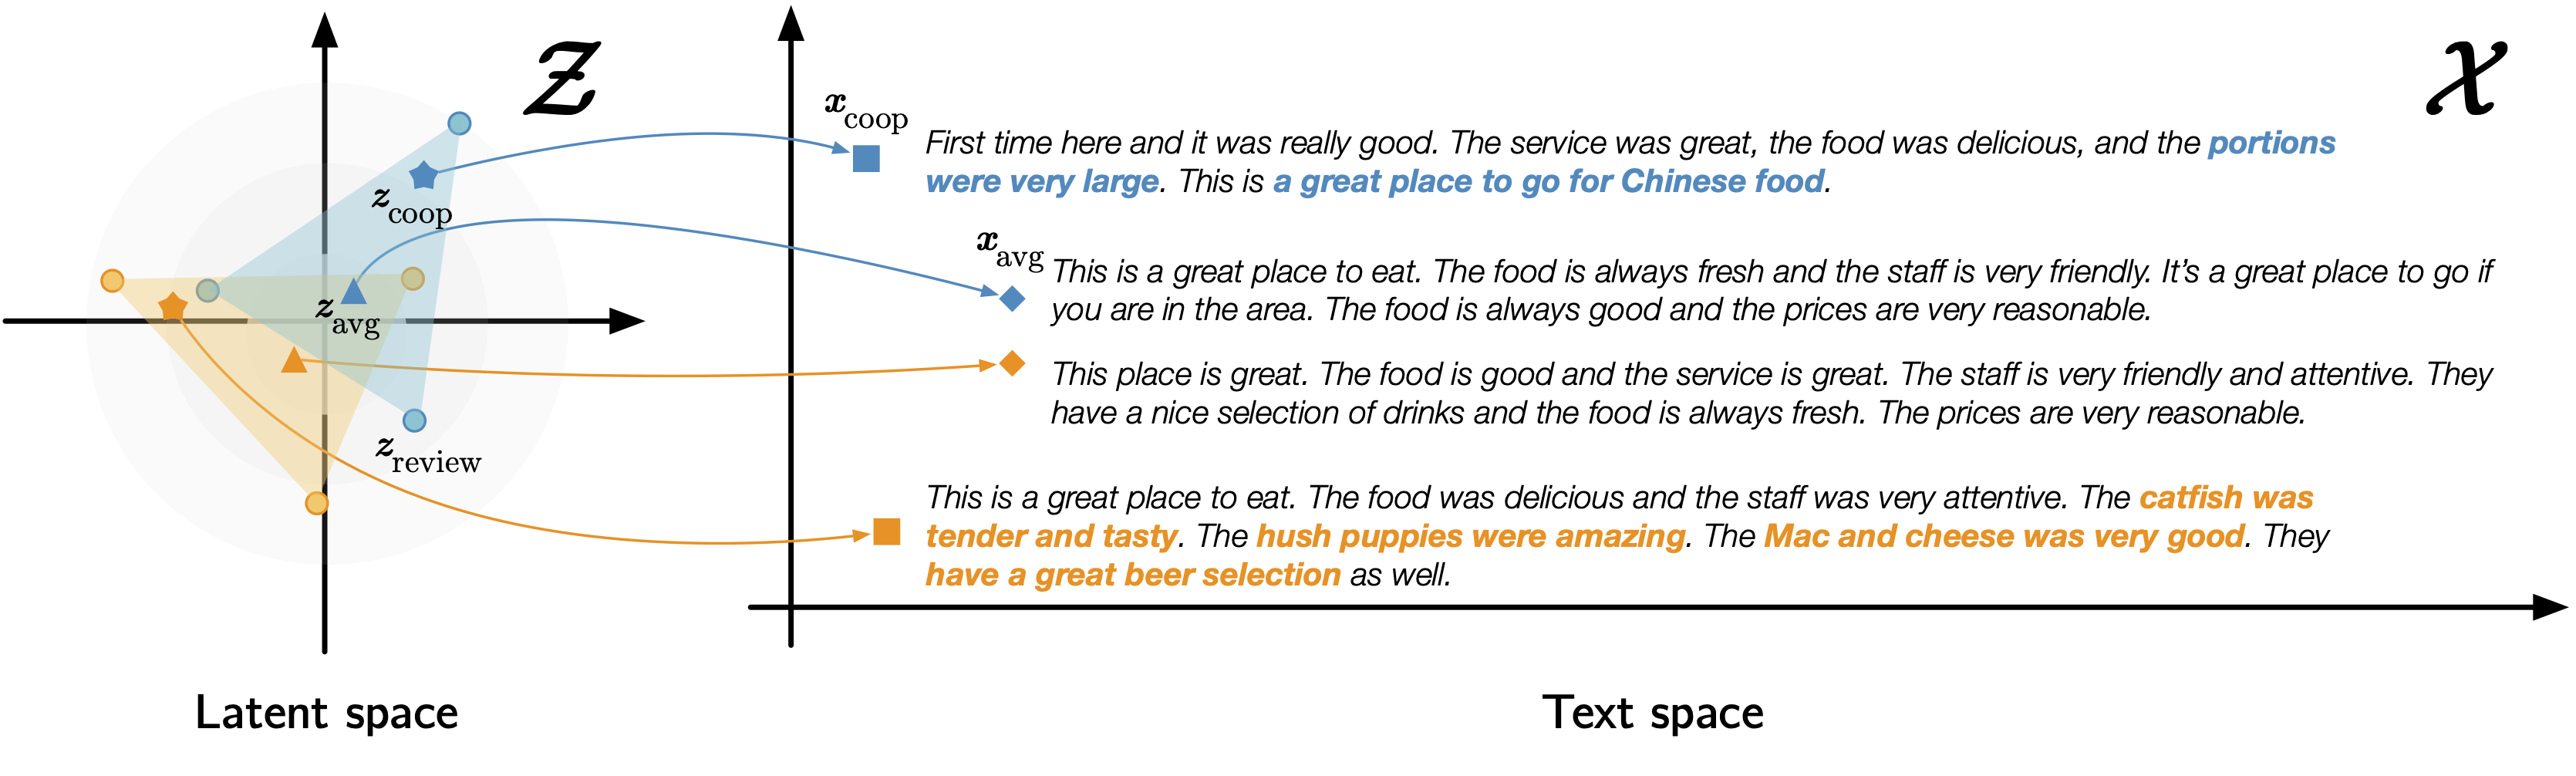
\includegraphics[width=\textwidth]{bilder/coop}
    \caption{Latentraum $Z$ mit den entsprechenden generierten Bewertungen $X$ \citep{coop}}
    \label{coop_fig}
\end{figure}

Wie in Abbildung \ref{coop_fig} zu erkennen ist ähneln sich Bewertungen, die durch Bestimmung des Durchschnitts der Latentvektoren generiert worden sind sehr. 
Auffällig ist die Korrelation zwischen der Ausdrucksstärke und dem Informationsgehalt eines Latentvektors und seiner $L_2$-Norm $\| z \|$.
Latentvektoren, die durch den Durschnitt bestimmt werden, haben eine geringere $L_2$-Norm und somit in den erzeugten Bewertungen einen geringeren Informationsgehalt \citep{coop}.

Um ausdrucksstarke Latentvektoren für die Generation der Bewertungen zu erhalten, formuliert COOP \citep{coop} die Bestimmung des optimalen Latentvektors als Optimierungsproblem, um die beste Kombination von einzelnen Latentvektoren zu finden.
\begin{alignat}{2}
    \max_z              &\quad&  Overlap(R_p, D_\theta(z))    & \\
    \text{unter der Nebenbedingung: } &\quad&  z = \sum_{i=1}^{|R_p|} w_i z_i \\
                         &\quad&  \sum_{i=1}^{|R_p|}w_i=1,                        &\quad \forall w_i \in \mathbb{R}^+
\end{alignat}
Maximiert wird der \textit{Input-Output-Word Overlap} zwischen den Eingabebewertungen $R_p$ und der generierten Bewertung $D_\theta(z)$. 
Die \textit{Overlap}-Metrik in Gleichung \ref{overlap_rouge} basiert auf dem ROUGE-1 F1 Score und ermöglicht es, Bewertungen zu generieren, die konsistent zu den Eingabebewertungen sind.
\begin{align}
    \label{overlap_rouge}
    Overlap(X,Y) = \text{ROUGE-1}_{F_1}(X,Y)
\end{align}

Die Suche der einzelnen Kombinationen wird auf die Potenzmenge der Eingabebewertungen $R_p$ beschränkt. 
Der Zusammenfassunslatentvektor $z_p$ wird anschließend aus dem Durchschnitt der ausgewählten Eingabebewertungslatentvektoren berechnet.
\begin{align}
z_p = \frac{1}{|R_p^{'}|} \sum_{i=1}^{R_p^{'}}z_i \text{, mit } R_p^{'} \in 2^{R_p} \setminus  \{ \emptyset\}
\end{align}
Die COOP Methode zur Kombination der einzelnen Latentvektoren, um ausdrucksstarke Bewertungen zu erhalten, erreicht State-of-the-Art Ergebnisse im Vergleich zu den anderen vorgestellten Methoden, die lediglich den normalen Durchschnittslatentvektor verwenden.
Die erzeugten Bewertungen sind repräsentativ für eine Gruppe von Bewertungen und erhalten ein hohes Maß an Informationen. 
Trotzdem stellt sich die Frage, ob und inwiefern sich diese Ergebnisse noch weiter optimieren lassen.
Im weiteren Verlauf wurde ein Verfahren entwickelt, welches entsprechende Latentvektoren weiterhin adaptiert, um ein noch höheres \textit{Input-Output-Overlapping} zu erhalten und somit präzisere Informationen in den Durchschnittsbewertungen zu generieren.

\pagebreak

\section{Controllable Generation mittels Gradientenverschiebung}\raggedbottom

\subsection{Gradientenverschiebung nach Bag of Words Klassifizierer}

\subsection{Kombiniert mit Beam Search}

\pagebreak

\section{Evaluierung der Modelle}\raggedbottom
Die unterschiedlichen Optimierungen der Latentvektoren für ein Optimus Modell werden auf dem Amazon und dem Yelp Datensatz verglichen und mit aktuellen State-of-the-Art Modellen in Relation gesetzt.
Es existieren im Dev-Datensatz jeweils 8 Eingabebewertungen und drei Gold-Summaries zum evaluieren der generierten Ausgabebewertungen.
Die Eingabebewertungen werden durch ein Optimus VAE Modell in Latentvektoren umgewandelt, welche anschließend mittels in Abschnitt \ref{coop} erklärter COOP Herangehensweise kombiniert werden, um den \textit{Input-Output-Overlap} zu maximieren. 
Weiterhin wird der Latentvektor mittels Attribut-Modell optimiert, um detailreichere Bewertungen zu erhalten.


\subsection{Evaluationsmetrik}
Die generierten Textbewertungen werden mit den drei Gold-Summaries verglichen.
Zum Vergleich der Bewertungen wird die \textbf{R}ecall-\textbf{O}riented \textbf{U}nderstudy for \textbf{G}isting \textbf{E}valuation (ROUGE) -Metrik verwendet.
Die ROUGE-N Metrik misst die Anzahl der übereinstimmenden N-Grams zwischen dem generierten Text und den Referenztexten. 
Ein "N-Gram" ist eine N-lange sequentielle Folge von Wörtern innerhalb der Texte. 

Zur Bewertung der generierten Bewertungen werden die vorhergesagten Ergebnisse mit den korrekten Ergebnissen verglichen. 
Die Konfusionsmatrix in Abbildung \ref{confusionmatrix} ist eine Wahrheitsmatrix, welche die Einteilung der vorhergesagten Ergebnisse ermöglicht. 
True Positive (TP) und True Negative (TN) sind von dem Modell korrekt vorhergesagte Ergebnisse, False Positive (FP) und False Negative (FN) ist eine Klasse von falsch vorhergesagten Ergebnissen.


\begin{figure}[h!]
    \centering
\begin{tikzpicture}[
    box/.style={draw,rectangle,minimum size=2cm,text width=1.5cm,align=left}]
    \matrix (conmat) [row sep=.1cm,column sep=.1cm] {
    \node (tpos) [box,
        label=left:Positive,
        label=above:Positive,
        ] {True \\ positive};
    &
    \node (fneg) [box,
        label=above:Negative] {False \\ negative};
    \\
    \node (fpos) [box,
        label=left:Negative] {False \\ positive};
    &
    \node (tneg) [box] {True \\ negative};
    \\
    };
    \node [left=.05cm of conmat,text width=1.5cm,align=right] {\textbf{Referenz}};
    \node [above=.05cm of conmat] {\textbf{Vorhersage}};
\end{tikzpicture}
\caption{Konfusionsmatrix}
\label{confusionmatrix}
\end{figure}
Zur Berechnung des ROUGE-N Scores werden die einzelnen Textabschnitte in eine Menge aus N-Grams zerlegt.
Mittels der Konfusionsmatrix in Abbildung \ref{confusionmatrix} lassen sich Precision (P) und Recall (R) definieren:
\begin{addmargin}[30pt]{30pt}
    \textbf{Precision}: 
    Der Precision Wert ergibt sich aus dem Verhältnis der korrekt vorhergesagten N-Grams und der Anzahl der insgesamt vorhergesagten N-Grams.
    \begin{align*}
    \text{P} = \frac{\text{TP}}{\text{TP}+\text{FP}}
    \end{align*}

    \textbf{Recall}:
    Recall ist als Verhältnis zwischen den korrekt vorhergesagten N-Grams und den N-Grams aus der Referenz definiert.
    \begin{align*}
    \text{R} = \frac{\text{TP}}{\text{TP}+\text{FN}}
    \end{align*}

    $\textbf{F}_1$:
    Das F1-Maß beschreibt das harmonische Mittel zwischen Precision und Recall.
    \begin{align*}
    \text{F}_{1} = \frac{2\text{PR}}{\text{P}+\text{R}}
    \end{align*}
\end{addmargin}

In der Evaluation werden die ROUGE-1, ROUGE-2 und ROUGE-L Werte miteinander verglichen.
ROUGE-1 verwendet als N-Gram Unigrams, ROUGE-2 Bigramme und ROUGE-L misst die längste gleiche Subsequenz zwischen Vorhersage und Referenz.

Da ROUGE-Scores lediglich die einzelnen Wortsequenzen miteinander vergleicht, findet die semantische Bedeutung und Ähnlichkeit der Bewertungen mit der Referenz keinen Einfluss.
Um trotzdem die semantische Ähnlichkeit zwischen Bewertungen und Referenz zu messen wird als weitere Metrik der Moverscore aus Abschnitt \ref{moverscore} verwendet.
Moverscore basiert auf BERT und vergleicht Context Embeddings mittels Earth-Mover-Distance. Als Metrik konnte der Moverscore hohe Korrelationen mit menschlichem Urteilsvermögen aufweisen.


\subsection{Bewertung der Datensätze}

\subsubsection{Amazon-Datensatz}

\subsubsection{Yelp-Datensatz}

\subsection{Ergebnisse}

\begin{table}[!h]
    \label{eval_results}
    \centering
    \begin{tabular}{@{}lllllllll@{}}
    \toprule
                               & \multicolumn{4}{c}{Amazon} & \multicolumn{4}{c}{Yelp} \\ 
    \textbf{Method} & \textbf{R1} & \textbf{R2} & \textbf{RL} & \textbf{MV} & \textbf{R1} & \textbf{R2} & \textbf{RL} & \textbf{MV}\\ \midrule
    \textit{Our Method}        &         &         &        &        &        &   & &     \\
    $\quad$ Optimus            &     \textbf{36.75}    &   \textbf{7.37}      &     \underline{20.60}  & &   \textbf{35.91}   &   \textbf{7.79}       & \underline{19.43}   &    \\ \midrule
    \textit{COOP}              &         &         &        &        &        & &   &    \\
    $\quad$ \textsc{BiMeanVae}$^{\star}$ & \underline{36.57}    & \underline{7.23}   & \textbf{21.24} & & \underline{35.37}  & \underline{7.35}  & \textbf{19.94} & \\
    $\quad$ Optimus $^{\star}$           & 35.32   & 6.22    & 19.84 & & 33.60  & 7.00   & 18.95 & \\ \midrule
    \textit{SimpleAvg}         &         &         &        &      &  &        &        \\
    $\quad$ \textsc{BiMeanVae}$^{\star}$ & 33.60   & 6.64    & 20.87 & & 32.87  & 6.93   & 19.89 & \\
    $\quad$ Optimus  $^{\star}$          & 33.54   & 6.18    & 19.34 & & 31.23  & 6.48   & 18.27 & \\
    $\quad$ MeanSum  $^{\star}$          & 29.20   & 4.70    & 18.15 & & 28.46  & 3.66   & 15.57 & \\
    $\quad$ CopyCat  $^{\star}$          & 31.97   & 5.81    & 20.16 & & 29.47  & 5.26   & 18.09 & \\ \midrule
    \textit{Extractive}        &         &         &        &      &  &        &  &      \\
    $\quad$ LexRank  $^{\star}$          & 28.74   & 5.47    & 16.75 & & 25.01  & 3.62   & 14.67 & \\ \bottomrule
    \end{tabular}
    \caption{ROUGE Ergebnisse auf den Benchmarkdatensätze der unterschiedlichen Modelle. Die besten Ergebnisse sind fett markiert und die zweitbesten Ergebnisse unterstrichen.
    $^{\star}$ denotiert, dass die Ergebnisse aus den Eregnissen von \citep{coop} übernommen wurden.}
\end{table}

\pagebreak

\section{Zusammenfassung und Ausblick}\raggedbottom
\label{summary}
In dieser Masterarbeit konnte ein umfassender Überblick über State-of-the-Art NLP-Techniken im Bereich der Multi-Document Summarization gegeben werden.
Es wurden unterschiedliche Architekturen wie Transformer, BERT, GPT-2, LSTM und Attention-Layer dargestellt. 
Insbesondere Variational Autoencoder, Optimierungen dieser Modelle und die Verwendung dieser Verfahren und Modelle im Bereich von Sprachmodellen wurde explizit erläutert.

Das Ziel dieser Arbeit war das Zusammenfassen von mehreren Rezensionen eines Produkts oder einer Dienstleistung zu einer generierten repräsentativen Rezension, die die anderen Rezensionen inhaltlich inkludiert und auf die verschiedenen wichtigen Aspekte der zu bewertenden Produkte oder Dienstleistung eingeht.
Hierzu wurde ein neuer Ansatz entwickelt.

Als Datensätze wurden Amazon- und Yelp-Review-Datensätze verwendet. Diese bieten eine Vielzahl an unterschiedlichen Rezensionen zu unterschiedlichen Produkten und Dienstleistungen. Insbesondere zur Multi-Review Summarization existieren menschlich erstellte Rezensionszusammenfassungen auf beiden Datensätzen.

Unterschiedliche extraktive und abstraktive Methoden wurden zur Multi-Review Summarization vorgestellt und untereinander verglichen. 
Die in dieser Arbeit als Grundlage verwendete Convex Aggregation for Opinion Summarization Methode basiert darauf, dass generierte Rezensionen aus normalen Durchschnittslatentvektoren ihre Expressivität verlieren. 
Die \textit{COOP} Methode findet eine optimale Kombination der einzelnen Latentvektoren für einen Durchschnittslatentvektor, um eine maximale Expressivität beizubehalten.

In dieser Masterarbeit wurde ein neuer Ansatz verfolgt, bei dem die \textit{COOP} Methode durch ein Bag of Words Attributmodell erweitert wird, um bei der Generierung von Rezensionen die berechneten Wahrscheinlichkeiten der Tokens in Bezug auf das gewählte Attributmodell zu optimieren.
Das Attributmodell wurde bei dem Optimus Modell in die Vergangenheitsmatrix von GPT-2 injiziert. Bei dem \textsc{BiMeanVAE} Modell wurde bei der Generierung jeweils der vorherige Zellzustand des LSTM-Decoders optimiert.

Durch Anwendung der Beam Search Methode auf den durch das Attributmodell optimierten Modelle konnten erfolgreich präzise Zusammenfassungen der Rezensionen generiert werden.
Des Weiteren wurde ein neuartiger Rankingalgorithmus zur Auswahl der besten generierten Rezension auf Basis der Kombination von mehreren ROUGE-Werten und dem Moverscore erstellt.

Das in dieser Masterarbeit entwickelte \textit{COOP}+Attributmodell zeigt eine hervorragende Performance bei der Zusammenfassung von Rezensionen. 
Die wichtigen Aspekte der unterschiedlichen Rezensionen werden wiedergegeben und insbesondere durch das Attributmodell zeigt sich eine Steigerung der Präzision bei den generierten Rezensionen. 
Im Vergleich zu den bisherigen Modellen übertrifft das \textit{COOP}+Attributmodell die Performance der anderen Modelle auf dem Amazon Datensatz in allen gewählten Metriken und erzielt hier State-of-the-Art Ergebnisse.
Auf dem Yelp Datensatz übertrifft das Optimus \textit{COOP}+Attributmodell die Referenzwerte.

Diese Ergebnisse bilden eine Grundlage für weiterführende Untersuchungen inwiefern Variational Autoencoder durch Verwendung von Attributmodellen bei der Generierung unterstützt werden können.
Ebenfalls wäre eine Auswertung der unterschiedlichen Methoden mittels menschlicher Evaluation sinnvoll, insbesondere auch um den Einfluss des Moverscore gestützten Ranking auf die empfundene Übereinstimmung von menschlichen Evaluatoren zu erörtern.
Somit könnte das in dieser Masterarbeit erstellte Modell kommerziell verwendet werden, um auf Webportalen Benutzern einen schnellen allgemeingültigen Überblick über unterschiedliche Rezensionen von Produkten und Dienstleistungen zu ermöglichen.



\pagebreak



%\section{Training von Optimus für Control Code Generation}\raggedbottom


\pagebreak

%%%%%%%%%%%%%%%%%%%%%%%%%%%%%%%%%%%%%%%%%%%%%%%%%%%%%%%%%%%%%%%%%%%%%%%%
%%%% ENDE TEXTTEIL %%%%%%%%%%%%%%%%%%%%%%%%%%%%%%%%%%%%%%%%%%%%%%%%%%%%%
%%%%%%%%%%%%%%%%%%%%%%%%%%%%%%%%%%%%%%%%%%%%%%%%%%%%%%%%%%%%%%%%%%%%%%%%

\clearpage

% Entfernen Sie das Kommentar aus der nachfolgenden Zeile, falls Sie einen Anhang in der Arbeit verwenden wollen. Beachten Sie, dass Sie sich im Verlauf der Arbeit mit \ref{...} (z.B. \ref{anhang:zusatz1}) auf den Anhang beziehen.
%\newpage
\appendix
\section{Anhang}

\subsection*{Zusatzteil 1} \label{anhang:zusatz1}

Dies ist ein Anhang.

\clearpage

\ifthenelse{\boolean{\biber}}{ %with biber do
	\DeclareNameAlias{sortname}{first-last}
	\printbibliography[heading=bibintoc, title=\references]
}{ %without biber do
	\bibliography{references}
	\bibliographystyle{science} %alphadin
	Variational}
%\vspace*{\fill}

\clearpage

\listoffigures

\listoftables

%\pagebreak

%\printindex
\end{document}